\documentclass[a4paper, twocolumn]{report}
\setlength{\columnsep}{2em}
\usepackage{float}
\usepackage{verbatim}
\usepackage[utf8]{inputenc}
\usepackage[italian]{babel}
\usepackage{amsmath}
\usepackage{mathtools}
\usepackage{amsbsy,amssymb,amsfonts, amsthm}
\usepackage[version=4]{mhchem}
\usepackage{graphicx}
\usepackage[left=2cm,right=2cm,top=2cm,bottom=2cm]{geometry}
\usepackage{xcolor}
\usepackage[hypertexnames=false]{hyperref}
\usepackage{nameref}
\usepackage{framed}
\usepackage[framemethod=TikZ]{mdframed}
\usepackage{appendix}
\usepackage{tikz}
\usetikzlibrary{math}
\usetikzlibrary{shapes,arrows}
\usepackage{pgfplots}
\usepackage{tcolorbox}
\usepackage{listings}
\usepackage{fancyhdr}
\usepackage{witharrows}

\newsavebox{\mybox}


\definecolor{myblue}{RGB}{0,163,243}
\renewcommand{\footrulewidth}{0.4pt}% default is 0pt

\pagestyle{fancy}
\fancyhf{}
\fancyhead[LE,RO]{\itshape\nouppercase{\rightmark}}
\fancyhead[RE,LO]{\itshape\nouppercase{\leftmark}}
\fancyfoot[LE,CO]{Sistemi Complessi}
\fancyfoot[LE,RO]{\thepage}


\newcounter{Sec}

\renewcommand*\thesection{\arabic{section}}

\newtcolorbox{redbox}[1]
{opacityback=1, colback=red!5!white,opacityframe=0.09, colframe=red!75!black,fonttitle=\bfseries, coltitle=black,title=#1}
\newtcolorbox{greenbox}[1]
{opacityback=1, colback=green!5!white,colframe=green!75!black, opacityframe=0.09,fonttitle=\bfseries,coltitle=black, title=#1}
\newtcolorbox{bluebox}[1]
{opacityback=1, colback=myblue!5!white,colframe=myblue!75!black,opacityframe=0.09, fonttitle=\bfseries,coltitle=black,title=#1}


\lstset{
      basicstyle=\ttfamily,
        columns=fullflexible,
	frame=single,
      	breaklines=true,
      	postbreak=\mbox{\textcolor{red}{$\hookrightarrow$}\space},
}

% figure support
\usepackage{import}
\usepackage{xifthen}
\pdfminorversion=7
\usepackage{pdfpages}
\usepackage{transparent}
\newcommand{\incfig}[1]{%
    \def\svgwidth{\columnwidth}
    \import{./figures/}{#1.pdf_tex}
}
\theoremstyle{plain}
\newtheorem{thm}{Theorem}[subsection] % reset theorem numbering for each chapter

\theoremstyle{definition}
\newtheorem{defn}{Definizione}[subsection] % definition numbers are dependent on theorem numbers
\newtheorem{exmp}{Esempio}[subsection]
\newtheorem{ex}{Esercizio}[subsection] % definition numbers are dependent on theorem numbers

\newcommand{\ffrac}[2]{\ensuremath{\frac{\displaystyle #1}{\displaystyle #2}}}
\newcommand{\angstrom}{\mbox{\normalfont\AA}}
\newcommand{\vect}[1]{\boldsymbol{#1}}
%\renewcommand{\[}{\begin{equation}}
%\renewcommand{\]}{\end{equation}}
\renewcommand{\theequation}{\thesection.\arabic{equation}}
\counterwithin*{equation}{section}
\newcommand{\rom}[1]{\uppercase\expandafter{\romannumeral #1\relax}}

% \xrightarrow[]{\mathcal{F}^{-1}}

\author{Edoardo Gabrielli}
\title{Sistemi complessi}
\begin{document}
\maketitle 
\tableofcontents

% Mindmap del corso
\chapter*{MindMap del corso}
\usetikzlibrary{mindmap,trees, backgrounds}
%\pagestyle{empty}
\begin{center}
\begin{tikzpicture}
  \path[mindmap,
      concept color=black,
      text=white,
      level 1 concept/.append style={level distance=160,sibling angle=90, scale = 1.1},
      level 3 concept/.append style={sibling angle=70, minimum size=0.5cm,  font=\fontsize{6pt}{9pt}\selectfont}]
  node[concept] (main) {Sistemi Complessi}
    [clockwise from=-30]
    child[concept color=green!50!black] {
      node[concept] (stoc) {Processi di stocastici}
      [clockwise from=90]
      child { node[concept] (mark) {Processi di Markov} }
      child { node[concept] (prob) {Probabilità} }
      child { node[concept] (SDE) {Calcolo stocastico (SDE) } }
      child { node[concept] (FK) {Fokker Plank}
	[clockwise from=-20]
	child[concept color=green!50!black] {
	   node[concept] (num1) {Metodi Numerici}
      	}
      }
      child { node[concept] (master) {Master equation e Jump Process}
      	[clockwise from=-70]
	child[concept color=green!50!black] {
	   node[concept] (stab) {Stabilità}
      	}
      }
    }  
    child[concept color=blue] {
      node[concept] (caos) {Sistemi caotici}
      [clockwise from=-90]
      child { node[concept] (Ham) {Sistemi Hamiltoniani} 
	[clockwise from=-30]
	child[concept color=blue] { node[concept] (kam) {KAM} }
	child[concept color=blue] { node[concept] (mel) {Melnikov} }
      }
      child { node[concept] (strum) {Strumenti} 
	[clockwise from=-80]
	child[concept color=blue] { node[concept] (poin) {Poincare} }
	child[level distance=2cm, concept color=blue] { node[concept] (mel) {Misure} }
      }
      child { node[concept] (diss) {Sistemi Dissipativi} }
    };
    \begin{pgfonlayer}{background}
	\draw (num1) to[circle connection bar switch color=from (green!50!black) to (green!50!black)] (SDE);
	\draw (strum) to[circle connection bar switch color=from (blue) to (blue)] (diss);
	\draw (strum) to[circle connection bar switch color=from (blue) to (blue)] (Ham);
    \end{pgfonlayer}
\end{tikzpicture}
\end{center}


\chapter{Processi stocastici}
\chapter{Processi stocastici}
\section{Introduzione ai processi di Markov}%
\label{sub:Lezione 1}
\mylocaltoc
\subsection{Ipotesi di Markov}%
\paragraph{Moto Browniano}
Il conte Brown nel 1827 pensò di aver scoperto la vita osservando particelle di polline in acqua che si muovevano in modo casuale, ne concluse che le particelle fossero vive. Successivamente fu Einstein a dare una descrizione collisionale con i seguenti punti chiave:
\begin{itemize}
    \item Impatti frequenti.
    \item Descrizione probabilistica.
    \item Dinamica discreta (tempo discretizzato).
\end{itemize}
Mettiamoci in un sistema unidimensionale e ipotizziamo che il tempo caratteristico di impatto tra due palline sia $\tau$ e che $n(t)$ sia il numero delle palline.\\
Sempre per ipotesi per ogni pallina si ha la proprietà:
\[
    x(t=0) = x \implies  x(t=\tau) = x + \Delta
.\] 
Dove $\Delta$ varia da pallina a pallina, possiamo definire una distribuzione pari di questi $\Delta$: $f(\Delta)$
\[\begin{aligned}
    &\int f(\Delta) d\Delta = 1; \quad &f(\Delta) = f(-\Delta) 
.\end{aligned}\]
\paragraph{Primo esempio di equazione di Fokker-Plank}%
Possiamo trovare il numero $dn$ di palline che si muovono di una quantità $\xi$: $\Delta < \xi < \Delta  + d\Delta$.
\begin{figure}[H]
    \centering
    \incfig{1-brown}
    \caption{\scriptsize Particelle che si muovono di $\xi$, dove $\Delta$ è la variabile stocastica per le palline.}
    \label{fig:1-brown}
\end{figure}
\noindent

\[
    dn = n f(\Delta) d\Delta
.\] 
La probabilità che una pallina si trovi nel punto $x$ al tempo $t+\tau$ per $dx$ è:
\begin{greenbox}{Equazione di Chapman-Kolmogorov}
 \begin{equation}
    P(x,t+\tau) dx = dx \int P(x-\Delta,t) f(\Delta) d\Delta \label{eq:CK_1}
\end{equation}
\end{greenbox}
\noindent
\begin{redbox}{Ipotesi di Markov}
    Un processo stocastico che evolve indipendentemente dal tempo si dice Markoviano. L'ipotesi d Markov afferma che l'espressione per la $P(x, t + \tau)$ non dipende da $t$.
\end{redbox}
\noindent
Espandendo in serie (di Kramers-Moyal) le probabilità:
\[\begin{aligned}
    &P(x, t+\tau) = P(x, t) + \frac{\partial P}{\partial t} \tau  \\
    & P(x-\Delta,t) = P(x,t) - \frac{\partial P}{\partial x} \Delta  + \frac{1}{2}\frac{\partial ^2 P}{\partial x^2} \Delta^2
.\end{aligned}\]
Si nota che lo sviluppo in $x$ viene troncato al secondo ordine mentre quello in $t$ solo al primo.
Inserendo nella \ref{eq:CK_1} infatti si ha che (per la parità della funzione $f$) il primo ordine in $x$ si annulla. Il risultato finale è un primo esempio di equazione del tipo Fokker-Plank:
\begin{equation}
    \frac{\partial P}{\partial t} = D \frac{\partial ^2P}{\partial x^2} \label{eq:FP_1}
\end{equation}
Nella quale $D$ vale:
\[
    D = \frac{1}{2\tau}\left<\Delta^2\right>
.\]    
Integrando la \ref{eq:FP_1} si ottiene, con le condizioni iniziali: $P(x,t=0) = \delta(x)$
\[
    P(x,t) = \frac{n}{\sqrt{4\pi Dt}}\exp\left(-\frac{x^2}{4Dt}\right)   
.\] 
\paragraph{Dinamica mesoscopica di Langevin}%
Per dinamica mesoscopica si intende una dinamica intermedia tra quella globale del sistema e quella "puntuale" (in questo caso della singola pallina di polline).\\
Invece che scrivere una equazione per la probabilità $P$ Langevin propose di partire dall'equazione di moto delle palline tenendo conto di:
\begin{itemize}
    \item Attrito: $-6\pi\eta d \dot{x}$ (Approccio alla Stokes) 
    \item Impatti random tra le altre particelle: $\xi$.
    \item Temperatura: $\left<mv^2/2\right> = kT/2$.
\end{itemize}
Si può scrivere la seguente equazione modello
\begin{equation}
    m\ddot{x} = -6\pi\eta d \dot{x} + \xi.
\end{equation}
Che è un primo esempio di equazione differenziale stocastica.\\
Se moltiplichiamo a destra e sinistra per $x$  possiamo riscriverla nel seguente modo:
\[
    \frac{1}{2}m\frac{\text{d} ^2}{\text{d} t^2}\left(x^2\right) - m\dot{x}^2 = -3\pi\eta d \frac{\text{d} }{\text{d} t}\left(x^2\right) + \xi x
.\] 
Possiamo mediare su tutte le possibili realizzazioni della $\xi$, se introduciamo l'ipotesi che gli impatti random siano scorrelati rispetto alla posizione dell'acqua $x$ si ha che:
\[
    \left<\xi x\right> = \left<\xi\right>\left<x\right> = 0 
\]
Questa ipotesi emerge sempre da una visione Markoviana secondo cui gli urti precedenti non incidono sugli urti successivi, il sistema così definito è un sistema senza memoria.
\[
    \frac{m}{2}\frac{\text{d} ^2}{\text{d} t^2} \left<x^2\right>-kT = -3\pi\eta d \frac{\text{d} }{\text{d} t} \left<x^2\right>
.\] 
Si risolve con metodi noti:
\[
    \frac{\text{d} }{\text{d} t} \left<x^2\right>=\frac{kT}{3\pi\eta d}+ C\exp\left(\frac{-6\pi\eta dt}{m}\right)
.\] 
Osservando solo la dinamica asintotica si trascura il termine esponenziale decrescente:
\begin{redbox}{Equazione di diffusione}
    \begin{equation}
       \left<x^2\right>_t-\left<x^2\right>_0 = \frac{kT}{3\pi\eta d}\cdot t
    \end{equation}
\end{redbox}
\noindent
Confrontando questa con l'equazione di Fokker-Plank della sezione precedente si ha una relazione tra $D$ ed i coefficienti di questa equazione:
\begin{bluebox}{Coefficiente di Einstein}
    \[
        D = \frac{kT}{6\pi\eta d}
    .\] 
    Detto anche coefficiente di diffusione.
\end{bluebox}
\subsection{Master equations}%
Le master equations si utilizzano per modellizzare processi "a salto" che coinvolgono variabili discrete, esempi di questi sistemi sono: la dinamica delle popolazioni o l'evoluzione del numero di infetti in un'epidemia.
\paragraph{Sistema di Lotka-Volterra}
Prendiamo un sistema in cui coesistono preda e predatore:
\begin{itemize}
    \item Conigli: $x$ 
    \item Volpi: $y$ 
\end{itemize}
L'evoluzione di $(x, y)$ può essere schematizzata con il seguente sistema (di Lotka-Voterra):
 \[
    \begin{cases}
	& x+\text{food}\to 2x\\
	& x+y\to 2y\\
	& y\to \text{death}
    \end{cases}
.\] 
Si introduce il parametro "food" come $c$ e si scrivono due equazioni differenziali per la variazione del numero di individui di ciascuna specie $x, y$:
\[
    \begin{cases}
	&\frac{\text{d} x}{\text{d} t} =k_1xc-k_2xy\\
	&\frac{\text{d} y}{\text{d} t} = k_2xy-k_3y
    \end{cases}
.\] 
Integrando numericamente tali equazioni emerge un andamento oscillatorio caratteristico di questo tipo di problemi (Figura \ref{fig:conigli}).
\begin{figure}[H]
    \centering
    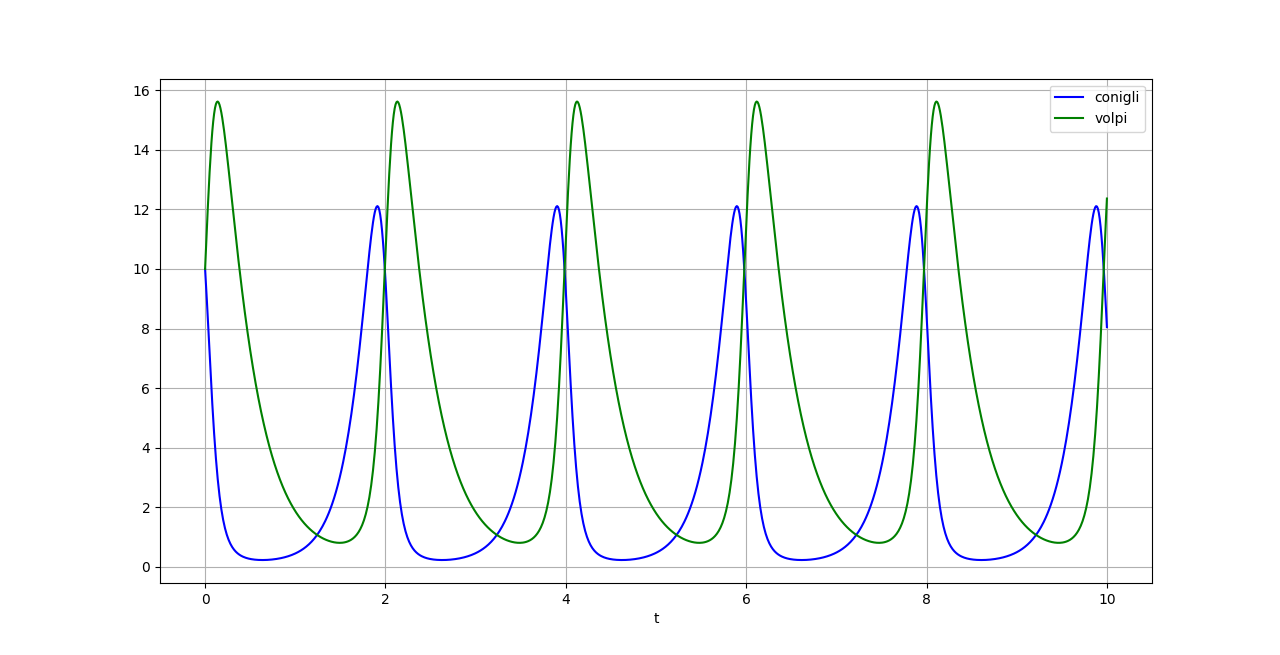
\includegraphics[width=0.4\textwidth]{figures/Volpi-Conigli.png}
\caption{\scriptsize Andamento delle soluzioni (\href{https://github.com/dodogabrie/Sistemi-Complessi/blob/master/python-project/lezione1/volpi_conigli.py}{Link al codice})}
    \label{fig:conigli}
\end{figure}
\noindent
Per una trattazione più rigorosa è necessario notare che le variabili in gioco non sono continue ma bensì discrete (numero di individui di popolazioni).\\
Si passa quindi ad una descrizione probabilistica del sistema che ci porta alla relativa Master Equation.
\begin{center}
    $P(\sigma, t) \in \mathbf{R}$: Probabilità di avere $\sigma \equiv (x,y)\in \mathbf{N}^2$ al tempo $t$.
\end{center}
Inseriamo l'ipotesi di Markov, ovvero che la probabilità che avvenga una transizione tra gli stati del sistema $\sigma \rightarrow \sigma'$ non dipenda dal tempo.
\begin{center}
    $P_r(\sigma\rightarrow\sigma')$: Probabilità di transizione indipendente da $t$.
\end{center}
Dato il sistema al tempo $t$ le probabilità di transizione in un intervallo $\Delta t$ sono:
\[\begin{aligned}
    &P_r(x\to x+1, y) = k_1 c x \Delta t\\
    &P_r(x\to x-1, y \to y+1) = k_2xy\Delta t\\
    &P_r(x\to x,y\to y-1) = k_3 y \Delta t\\
    &P_r(x\to x,y\to y) = 1 - \Delta t \left(k_1cx+ k_2xy + k_3 y\right)
.\end{aligned}\]
Possiamo esprimere la variazione nel tempo della distribuzione di probabilità $P$ tramite le quantità $P_r$:
\begin{redbox}{Esempio di Master Equation}
    Si usa la semplificazione $x^{\pm} \equiv x \pm 1$.
    \begin{equation}
        \begin{aligned}
	    &\frac{P(x,y,t+\Delta  t) - P(x,y,t)}{\Delta  t}  =\\
	    & \quad P_r(x^-\to x, y) \cdot P(x^-,y,t) +\\
	    & \quad P_r(x^+\to x, y^-\to y) \cdot P(x_+,y^-,t) + \\
	    & \quad P_r(x\to x, y^+\to y) P(x,y^+,t) + \\
	    & \quad - \left[1-P_r(x\to x, y\to y)\right]\cdot P(x,y,t) 
        \end{aligned}
    \end{equation}
\end{redbox}
\noindent
Il termine di destra esprime la probabilità di ingresso nello stato $\sigma = (x,y)$ meno la probabilità di uscita da tale stato.
\paragraph{Modello SIR}
Il modello SIR può essere utilizzato per descrivere una situazione pandemica. Gli individui di una popolazione presi in analisi sono:
\begin{itemize}
    \item Suscettibili: $S$.
    \item Infetti: $I$.
    \item Immuni (dopo la malattia): $R$.
\end{itemize}
\[
    \begin{cases}
    S_{n+1} = S_n - \alpha S_n I_n \Delta t\\
    I_{n+1} = I_n + (\alpha S_n I_n - \gamma I_n) \Delta t\\
    R_{n+1} = R_n + \gamma I_n \Delta t
    \end{cases}
\]
Per scrivere la Master Equation si osserva quali sono i termini guidano le transizioni tra i vari stati del sistema:
\[\begin{aligned}
    &P_r(S\to S^-, I \to I^+, R) = \alpha S I \Delta t\\
    &P_r(S, I \to I^-, R \to R^+) = \gamma I \Delta t
.\end{aligned}\]
In modo analogo a quanto fatto per l'esempio precedente si arriva alla seguente equazione:

\begin{align*}
    P(\sigma, &t + \Delta t) = P(\sigma, t) + \\
     + \Delta t &\left[ P(S^+, I^-, R, t) P_r(S^+\to S, I^- \to I, R) + \right.\\
		& \left.+ P(S, I^+, R^-, t) P_r(S, I^+ \to I, R^-\to R) \right] + \\
     - \Delta t & P(\sigma, t) \left[ P_r(S\to S^-, I \to I^+, R) \right. + \\
		& \qquad \qquad \left.+ P_r(S, I\to I^-, R\to R^+)\right].
\end{align*}
A differenza del caso precedente questo sistema ha una configurazione di equilibrio (quando tutti hanno preso il COVID-19 ad esempio).
\paragraph{Rumore shot}%
Ipotizziamo di avere un cavo di rame attraversato da corrente elettrica $J$ e chiamiamo $\sigma$ una sezione di tale cavo ortogonale alla direzione di $J$. Il numero di elettroni che attraversano $\sigma$ sarà soggetto a fluttuazioni, tali fluttuazioni caratterizzano il rumore Shot.\\
La variabile stocastica del problema è $t_k$: il tempo di arrivo di un elettrone su $\sigma$. Ogni elettrone contribuisce alla corrente (misurata su $\sigma$) di una quantità che possiamo schematizzare come una scarica di condensatore $F(t-t_k)$:
\[
    F(t) = \begin{cases}
	0	 			&t<0\\
	q \exp\left(-\alpha t\right) 	&t \ge 0
    \end{cases}
\] 
La corrente totale sarà data dalla somma degli elettroni che arrivano su $\sigma$ per ciascun tempo stocastico $t_k$:
\[
    I(t) = \sum_{t_k}^{} F(t-t_k) 
.\] 
Cerchiamo la Master equation per questo sistema, partiamo dall'ipotesi che in un dato intervallo di tempo $\Delta t$ la probabilità che il numero di elettroni che attraversano $\sigma$ passi da $n$ a $n+1$ sia:
\[
    P(n\to n+1, \text{nell'intervallo }\Delta  t) = \lambda \Delta t
.\] 
Notiamo che gli elettroni scorrono in un'unica direzione, quindi il numero di elettroni che attraversa $\sigma$ può solo aumentare.\\
Il termine della Master Equation $P(n, t + \Delta t)$ si scrive come somma di:
\begin{itemize}
    \item Probabilità di avere già $n$ elettroni al tempo $t$ e che nell'intervallo $\Delta t$ non succeda niente:
	\[
	    (1-\lambda \Delta t) P(n, t)
	\]
    \item La probabilità che al tempo $t$ si hanno $n-1$ elettroni e che nell'intervallo $\Delta t$ ne arrivi un altro:
	\[
	    \lambda \Delta t P(n-1, t)
	\]
\end{itemize}
Quindi mettendo tutto insieme:
\[
    P_n(t+\Delta  t) = \left(1-\lambda\Delta t\right)P_n(t) + \lambda\Delta t  P_{n-1}(t)\implies 
\] 
\[
	\frac{P(n, t+\Delta  t) - P(n,t)}{\Delta t} = \lambda\left[P(n-1,t) -P(n,t)\right] 
.\] 
Che è proprio l'equazione cercata. Vediamo adesso un metodo di risoluzione di questo tipo di equazione.

%%%%%%%%%%%%%%%%%%%%%%%%%%%%%%%%%%%%%%%
%  Metodo della funzione generatrice  %
%%%%%%%%%%%%%%%%%%%%%%%%%%%%%%%%%%%%%%%
\subsection{Metodo della funzione generatrice}%
\label{subsec:fgen_met}
Per risolvere il problema introduciamo la funzione generatrice $G(s,t)$:
\[
    G(s,t) =\sum_{n}^{} s^nP(n,t) 
.\] 
Sostituendo nella master equation del problema precedente nel limite di $\Delta t \to 0$ si ha:
\[
    \frac{\partial G(s,t)}{\partial t} = \lambda (s-1) G(s,t)
.\] 
\[
     \implies  G(s,t) = \exp\left(\lambda (s-1) t\right)G(s,0) 
.\] 
Gli elettroni arrivano per $t\ge 0$, infatti si deve avere che: 
\[
    \begin{cases}
	&P(0,0)=1\\
	&P(n,0) = 0
    \end{cases}
    \ \forall n \implies  G(s,0) = 1 
.\] 
\[\begin{aligned}
    &G(s,t) = e^{\lambda (s-1) t} = \sum_{}^{} s^n P(n,t) \implies  \\
    &\sum e^{-\lambda t} e^{\lambda s t} = \sum_{}^{} e^{-\lambda t}\frac{\left(\lambda ts\right)^n }{n!}  = \sum_{}^{} s^nP(n,t) 
.\end{aligned}\]
In cui si è sfruttato la serie dell'esponenziale $e^{\lambda st}$.
\begin{redbox}{Distribuzione di Poisson}
    \[
	P(n,t)= e^{-\lambda t}\frac{\left(\lambda t\right)^{n}}{n!}
    .\] 
    Dove $P(n,t)$ è la probabilità che al tempo $t$ ci siano $N(t) =n$ elettroni nel sistema.
\end{redbox}
\noindent
Procediamo con il calcolo della corrente, se $N$ è il numero di elettroni arrivati all'istante $t$ allora possiamo definire la quantità:
\[
    \mu(t) \equiv 
    \frac{\text{d} N}{\text{d} t} 
    = \sum_k\delta (t-t_k)  
\] 
Dove $t_k$ è il tempo (random) in cui arriva un elettrone.
Passiamo al continuo nei tempi di arrivo degli elettroni e riscriviamo la corrente come:
\[\begin{aligned}
    I(t) =& \int dx F(t-x) \mu(x) =\\
	 =&\int_{- \infty}^{t} q \exp\left(-\alpha (t-x) \right) \frac{\text{d} N}{\text{d} x} dx 
.\end{aligned}\]
La difficoltà dell'espressione sta nel fatto che $N(t)$ è una funzione a gradini con i gradini che arrivano in modo stocastico nel tempo.\\
Si deriva a destra e sinistra rispetto al tempo ed si integra per parti:
\[\begin{aligned}
    \frac{\text{d} I}{\text{d} t} &= \left[q\exp\left(-\alpha (t-x)\right)\left. \frac{\text{d} N}{\text{d} t}\right]  \right|_{x=t} + \\
				   &\qquad +\int_{-\infty}^{t} \left(-\alpha q\right)\exp\left(-\alpha (t-x)\right)\frac{\text{d} N}{\text{d} x} dx =\\
				   &= q\mu (t) - \alpha I(t) 
.\end{aligned}\]
\begin{redbox}{Equazione stocastica differenziale}
 \[
    \frac{\text{d} I}{\text{d} t} = -\alpha I(t) + q\mu (t) 
.\]    
\end{redbox}
\noindent
Il termine in $\mu$ dipende dalla sequenza casuale di $\delta(t-t_k)$, ognuna di queste può dare soluzioni differenti.\\ 
Rispetto al moto Browniano visto in precedenza, in cui si aveva che $f(\Delta) = f(-\Delta)$, adesso abbiamo un processo che evolve solo in avanti.\\
L'idea per risolvere il problema è di interpolare l'andamento di $N$ con un moto browniano, prendendo la media e le fluttuazioni del termine stocastico.
Essendo il termine in $\mu$ la derivata di un processo poissoniano abbiamo le seguenti proprietà:
\[\begin{aligned}
    &\left<\mu dt\right>=\left<dN\right> = \lambda dt\\
    & \left<\left(\lambda dt - \mu dt\right)^2\right> = \lambda dt
.\end{aligned}\]
Si cerca di scrivere questo processo stocastico (unilaterale) come un processo di Langevin, quindi si definisce una nuova variabile stocastica $d\eta = dN - \lambda dt$.
\[
    dN = \lambda dt + d\eta	
.\] 
Questo equivale a scomporre il processo a salti $dN$ in un drift lineare ($\lambda dt$) ed una fluttuazione stocastica ($d\eta$).\\
Il differenziale della corrente si scrive come:
\[
    dI(t) = \left(\lambda q-\alpha I\right)dt+ qd\eta (t) 
.\] 
In questo modo la variabile stocastica $d\eta$ gode delle seguenti proprietà:
\begin{itemize}
    \item $\left<d\eta \right> = 0$
    \item $\left<d\eta^2 \right> = \lambda dt$
    \item $\left<I d\eta \right> = 0$
\end{itemize}
\[
    \frac{\text{d} }{\text{d} t} \left<I\right> = \lambda q -\alpha\left<I\right>
.\] 
Il risultato stazionario per l'equazione è:
\[
    \left<I\right>_{\infty}=\frac{\lambda q}{\alpha}
.\] 
Procediamo con una ipotesi sbagliata: trascurare le fluttuazioni nel seguente termine
\begin{equation}
    \left(I+dI\right)^2 \approx I^2 + 2IdI	\label{eq:baddiff}
\end{equation}
Quindi con il risultato che dovrebbe esser noto sui differenziali: $d\left(I^2\right) = 2IdI$, se assumiamo questo e moltiplichiamo a destra e sinistra per $\left<I\right>$ nella equazione   per la corrente otteniamo:
\[
    \frac{1}{2}\frac{\text{d} }{\text{d} t} \left<I^2\right>= \lambda q\left<I\right>-\alpha\left<I^2\right>
.\] 
Che ci porta a concludere che:
\[
    \left<I^2\right>_{\infty} = \frac{\lambda q}{\alpha}\left<I\right>_{\infty} = \left(\left<I\right>_{\infty}\right)^2
.\] 
Otteniamo quindi un paradosso, la corrente ha varianza nulla:
\[
  \left<I^2\right>-\left<I\right>^2 = 0  
.\] 
Questo significherebbe che la "larghezza" del moto Browniano è nulla, quindi la corrente sarebbe costante e continua.\\
L'errore è dovuto al differenziale \ref{eq:baddiff}, infatti il termine trascurato vale:
\[
    \left<dI^2\right> = \left<q^2d\eta^2\right> = q^2\lambda dt
.\] 
Che è anch'esso di prim'ordine nel tempo! L'equazione corretta sarebbe allora:
\[
    \frac{1}{2}\frac{\text{d} }{\text{d} t} \left<I^2\right>= \lambda q\left<I\right>-\alpha\left<I^2\right> + q^2\lambda + O(dt)
.\]
\newpage

\section{Lezione 2}%
\label{sub:Lezione 2}

\subsection{Esempi di Master equation}%
\begin{itemize}
    \item Rumore shot.
    \item Rumore Jonshon
\end{itemize}
Prendiamo il rumore Shot, questo si basa sul fatto che la corrente non è proprio continua, chiamiamo $t_k$ il tempo di arrivo di un elettrone:
\[
    I(t) = \sum_{t_k}^{} F(t-t_k) 
.\] 
Mentre $F(t-t_k)$ è una funzione a pinna di squalo. Cerchiamo la Master equation per questo sistema:
\[
    P(n\to n+1, \text{in }\Delta  t) = \lambda \Delta tP_n(t) 
.\] 
Visto che possiamo riscrivere la probabilità di avere $n$ elettroni al tempo $t+\Delta t$ come: 
\[
    P_n(t+\Delta  t) = \left(1-\lambda\Delta t\right)P_n(t) + \lambda\Delta t 
.\] 
Si ottiene:
\[
    \frac{P(n, t+\Delta  t) - P(n,t)}{\Delta t} = \lambda (P(n-1,t) -P(n,t)) 
.\] 
\subsection{Metodo della funzione generatrice}%
Possiamo risolvere questa equazione utilizzando una tecnica standard: la funzione generatrice $G(s,t)$:
\[
    G(s,t) =\sum_{}^{} s^nP(n,t) 
.\] 
Sostituendo nella master si ha:
\[
    \frac{\partial G(s,t)}{\partial t} = \lambda (s-1) G(s,t) 
.\] 
Che si risolve con il risultato:
\[
    G(s,t) = \exp\left(\lambda (s-1) t\right)G(s,0) 
.\] 
Gli elettroni arrivano per $t\ge 0$, infatti si deve avere che: $P(0,0)=1$, $P(n,0) = 0 \ \forall n$, queste condizioni iniziali ci portano a $G(s,0) = 1$.
\[\begin{aligned}
    G(s,t) =& e^{\lambda (s-1) t}G(s,0) = \sum_{}^{} s^n P(n,t) \implies  \\
		&\sum_{}^{} e^{-\lambda t}\frac{\left(\lambda ts\right)^n }{n!}G(s,0)  = \sum_{}^{} s^nP(n,t) 
.\end{aligned}\]
In cui si è sfruttato la serie dell'esponenziale $e^{\lambda st}$.
\begin{redbox}{Distribuzione di Poisson}
    \[
	P(n,t)= e^{-\lambda t}\frac{\left(\lambda t\right)^{n}}{n!}
    .\] 
    Dove $P(n,t)$ è la probabilità che al tempo $t$ abbiamo $N(t) =n$ elettroni.
\end{redbox}
\noindent
Tornando alla corrente dobbiamo trovare un modo per contare gli elettroni:
\[
    \mu (t) = \frac{\text{d} N}{\text{d} t} \quad
    \begin{cases}
	&0 \quad \text{di solito}\\
	&\delta (t-t_k) \quad \text{Arriva e$^-$ al tempo }t_k
    \end{cases}
\] 
Dove ricordiamo che $t_k$ è random.
Quindi abbiamo che: 
\[
    \mu (t) = \sum_{k}^{} \delta (t-t_k) 
.\] 
Allora possiamo riscrivere la corrente con un integrale sfruttando le $\delta$:
\[
    I(t) = \int dx F(t-t_k) \mu (x) 
.\] 
Prendendo come $F$ modello la funzione:
\[
    F(t) = \begin{cases}
        0 \quad t<0\\
	q \exp\left(-\alpha t\right) \quad t \ge 0
    \end{cases}
.\] 
Otteniamo per la corrente:
\[
    I(t) = \int_{- \infty}^{t} q \exp\left(-\alpha (t-x) \right) \frac{\text{d} N}{\text{d} x} dx 
.\] 
Adesso dobbiamo risolvere il problema che $N(t)$ è una funzione a salti irregolari tra loro. Vediamo l'equazione differenziale per $I(t)$.
\[\begin{aligned}
    \frac{\text{d} I}{\text{d} t} =& q\exp\left(-\alpha (t-x)\right)\left.\dot{N}\right|_{x=t} + \\
				   &+\int_{-\infty}^{t} \left(-\alpha q\right)\exp\left(-\alpha (t-x)\right)\dot{N}dx 
.\end{aligned}\]
Risolvendo a sinistra ed usando le definizioni ci si riduce a:
\begin{redbox}{Equazione stocastica differenziale}
 \[
    \frac{\text{d} I}{\text{d} t} = -\alpha I(t) + q\mu (t) 
.\]    
\end{redbox}
Il termine in $\mu$ dipende dalla sequenza casuale di $\delta$, ogni sequenza casuale diversa ci può dare soluzioni diverse.\\
L'idea per risolvere il problema è di interpolare l'andamento di $N$ con un moto browniano, prendendo la media e le fluttuazioni del termine stocastico.
Essendo il termine in $\mu$ la derivata di un processo poissoniano abbiamo le seguenti proprietà:
\[\begin{aligned}
    &\left<\mu dt\right>=\left<dN\right> = \lambda dt\\
    & \left<\left(\lambda dt - \mu dt\right)^2\right> = \lambda dt
.\end{aligned}\]
Si ha un termine di fluttuazioni $d\eta$ tale che:
\[
    dN = \lambda dt + d\eta	
.\] 
Il differenziale della corrente si scrive come::
\[
    dI(t) = \left(\lambda q-\alpha I\right)dt+ qd\eta (t) 
.\] 
Prendendo la media di questa equazione abbiamo che il termine di fluttuazione media a zero:
\[
    \frac{\text{d} }{\text{d} t} \left<I\right> = \lambda q -\alpha\left<I\right>
.\] 
Questa equazione per tempi lunghi da il risultato stazionario:
\[
    \left<I\right>_{\infty}=\frac{\lambda q}{\alpha}
.\] 
Andiamo avanti nel conto con la seguente presa di posizione:
\begin{equation}
    \left(I+dI\right)^2 \approx I^2 + 2IdI	\label{eq:baddiff}
\end{equation}
Quindi con il risultato che dovrebbe esser noto sui differenziali: $d\left(I^2\right) = 2IdI$, se assumiamo questo e moltiplichiamo a destra e sinistra per $\left<I\right>$ nella equazione   per la corrente otteniamo:
\[
    \frac{1}{2}\frac{\text{d} }{\text{d} t} \left<I^2\right>= \lambda q\left<I\right>-\alpha\left<I^2\right>
.\] 
Che ci porta a concludere che:
\[
    \left<I^2\right>_{\infty} = \frac{\lambda q}{\alpha}\left<I\right>_{\infty} = \left(\left<I\right>_{\infty}\right)^2
.\] 
Otteniamo quindi un paradosso, la corrente ha varianza nulla:
\[
  \left<I^2\right>-\left<I\right>^2 = 0  
.\] 
Questo significherebbe che la "larghezza" del moto Browniano è nulla, quindi la corrente sarebbe costante e continua.\\
L'errore è dovuto al differenziale \ref{eq:baddiff}, infatti il termine trascurato vale:
\[
    \left<dI^2\right> = \left<q^2d\eta^2\right> = q^2\lambda dt
.\] 
Che è anch'esso di prim'ordine nel tempo! L'equazione corretta sarebbe allora:
\[
    \frac{1}{2}\frac{\text{d} }{\text{d} t} \left<I^2\right>= \lambda q\left<I\right>-\alpha\left<I^2\right> + q^2\lambda
.\]

\section{Funzione caratteristica e Momenti Fattoriali}%
\label{sub:Lezione 3}
\mylocaltoc
\subsection{Funzione caratteristica e cumulanti}%
\label{sub:Funzione caratteristica}
Sia $\vect{x}$ una variabile random con distribuzione di probabilità $P(\vect{x})$, la funzione caratteristica della distribuzione è la sua trasformata di Fourier:
\begin{redbox}{}
    \[
	\phi (\vect{s}) = \int d\vect{x} P(\vect{x}) e^{i \vect{x}\cdot \vect{s}}
    .\] 
\end{redbox}

\begin{exmp}[Distribuzione Gaussiana]
 \[\begin{aligned}
    &P(x) = \frac{e^{-x^2 / 2 \sigma^2}}{\sqrt{2\pi\sigma^2}} 
    &\implies&
    &\phi (s) = e^{-\sigma^2s^2 / 2}
.\end{aligned}\]
\end{exmp}

\begin{exmp}[Distribuzione uniforme]
\[
    P(x) = 
    \begin{cases}
	1 & x \in \left[-\frac{1}{2}, \frac{1}{2}\right]\\
	0 & \text{Altrimenti}
    \end{cases}
\] 
\[
    \phi (s) = \int_{-1 /2}^{1 /2} e^{ixs}dx = \frac{2}{s}\sin\left(\frac{s}{2}\right)  
.\] 
\end{exmp}

\subsubsection{Proprietà della funzione caratteristica}%
\label{ssub:Proprietà della funzione caratteristica}
\begin{enumerate}
    \item $\left|\phi (0) \right|= 1 $.
    \item $\phi (s) $ è continua.
    \item Se $\exists \left<x^n\right>$ allora: 
	\[
		\left<x^n\right> = \left(-i\right)^n \left.\frac{\partial ^n}{\partial s^n} \phi (s)\right|_{s=0} 
	.\] 
    \item Una sequenza di distribuzioni converge ad una distribuzione limite $\iff$ converge la sequenza di funzioni caratteristiche.
    \item Dato $\vect{x} = \left(x_1, \ldots, x_n\right)$ con $x_i$ indipendenti $\forall i$ allora:
	\[ 
	    \phi (s_1, s_2, \ldots) = \prod_{i=1}^{n} \phi (s_i)  
	\]
    \item Se $y = \sum_{i}^{} x_i$ con $x_i$ indipendenti, allora:
	\[
	    \phi (s) = \left<e^{isy}\right> = \prod_{i}^{} \phi_i(s)  
	.\] 
	\begin{exmp}
	    Se $y = x_1 + x_2$ ho che:
	    \[
		P(y) = \int P(x_1) P(y-x_1) dx_1
	    .\] 
	    Allora per le proprietà della trasformata di una convoluzione:
	    \[
		\phi (s) = \phi_1(s) \phi_2(s) 
	    .\] 
	\end{exmp}
\end{enumerate}
\begin{exmp}[Testa o Croce]
    Prendiamo una distribuzione che corrisponda alla probabilità del set di eventi ["testa","croce"] dopo il lancio di una moneta:
    \[
        P(x) = \frac{1}{2}\left( \delta(x-1) + \delta(x+1) \right) 
    \]
    Calcoliamo la funzione caratteristica di tale distribuzione:
    \[
	\phi(s) = \int P(x) e^{isx} dx = \frac{1}{2}\left[ e^{is} + e^{-is} \right] 
    \]
    Ipotizziamo di fare $n$ lanci di moneta e di voler inferire tramite la funzione caratteristica quale sarà la distribuzione di probabilità finale. \\
    Stiamo parlando della probabilità di una somma di eventi indipendenti, quindi per quanto visto in precedenza si ha che:
    \[
	\phi_n(s) = \left[ \phi(s) \right] ^n = \frac{1}{2^n} \left( e^{is} + e^{-is} \right)^n 
    \]
    Si sfrutta la formula binomiale (somma di elementi elevati alla $n$):
    \[
	\phi_n(s) = \frac{1}{2^n}\sum_{k = 0}^{n}\binom{n}{k} e^{is(n-2k)}
    \]
    La trasformata inversa assume la forma di una somma di delta di Dirac che dovrebbero convergere ad una Gaussiana nel limite di $n\to\infty$:
    \[
	P(x) = \frac{1}{2\pi}\int ds \phi_n(s) e^{-ixs} = \frac{1}{2^n} \sum_{k = 0}^{n} \binom{n}{k}\delta(n-2k)
    \]
\end{exmp}
\subsubsection{Cumulanti della funzione caratteristica.}%
\label{sub:Sviluppo in cumulanti di phi}
\begin{redbox}{Funzione generatrice dei cumulanti}
   \[
       \Phi(s) = \ln (\phi (s) ) 
   .\]  
\end{redbox}
\noindent
Si potrebbe dimostrare che la funzione generatrice si esprime in modo generale in funzione di quantità definite come cumulanti:
\[\begin{aligned}
    \Phi = \sum_{r=1}^{\infty} i^r \sum_{\left\{m\right\}}^{} 
    \left<\left< x_1^{m_1}x_2^{m_2}\ldots\right>\right> 
    \prod_{i=1}^{\infty} \frac{s_i^{m_i}}{m_i!\,}\delta (r-\sum_{i=1}^{r} m_r) 
.\end{aligned}\]
Dove i termini tra le parentesi $\left<\left< x_i^{m_i}\right>\right>$ sono i cumulanti. Prendiamo ad esempio lo sviluppo dei primi due:
\[\begin{aligned}
    & \left<\left<x_1\right>\right> = \left<x_1\right> \sim \text{Media}\\
    & \left<\left<x_1 x_2 \right>\right> = \left<x_1x_2\right> - \left<x_1\right>\left<x_2\right> \sim \text{ Covarianza}
.\end{aligned}\]
Consideriamo adesso i cumulanti per una stessa variabile stocastica ($x_i = x_j $ $\forall i, j$), che chiameremo in questo contesto anche \texttt{Momenti}.
\begin{greenbox}{Cumulanti di processo Gaussiano.}
   I cumulanti per un processo Gaussiano sono tutti nulli per $n\ge 3$.
   \[
       \left<\left<x^n\right>\right> = 0 \quad \forall n \ge  3
   .\] 
\end{greenbox}
\begin{exmp}[Cumulante quarto per Gaussiana]
    \[\begin{aligned}
	\left<\left<x^4\right>\right> =& \left<x^4\right>-4\left<x^3\right>\left<x\right>+\\
					&-3\left<x^2\right>^2 + 12\left<x^2\right>\left<x\right>^2-6\left<x\right>^4
    .\end{aligned}\]
    Possiamo dimostrare che $\left<\left<x^4\right>\right> = 0$ valutando $\frac{d}{dx}\left<x^3\right>$:
    \[
        \int_{-\infty}^{\infty} \frac{\text{d} }{\text{d} x} \left\{x^3 \exp\left(\frac{-x^2}{2\sigma^2}\right)\right\} dx = 0 
    .\] 
    Questa si azzera perché la Gaussiana si annulla in $x = \pm \infty$, la precedente equazione può essere riscritta tramite le regole della derivata composta:
    \[
        \int\left(3x^2\exp\left(-\frac{x^2}{2\sigma^2}\right) - 
		\frac{x^4}{\sigma^2}\exp\left(- \frac{x^2}{2\sigma^2}\right) \right)dx = 0 
    .\] 
    \[
	\left<x^4\right> = 3\sigma^2\left<x^2\right> = 3 \left(\sigma^2\right)^2
    .\] 
    Inserendo nella equazione per il cumulante quarto si annullano tutti i termini (per semplicità abbiamo preso una gaussiana a media nulla $\left<x\right>=0$ ) .
\end{exmp}
\noindent
In generale questa cosa non funziona, non è possibile esprimere i cumulanti in funzione di altri cumulanti di ordine inferiore per ogni distribuzione.

\subsection{Teorema del limite centrale}%
\label{sub:Teorema del limite centrale}
\begin{redbox}{Teorema del limite centrale}
   La somma di variabili stocastiche aventi media e varianza definita tende ad una Gaussiana. 
\end{redbox}
\noindent
Sia $\left\{x_i\right\}$ una variabile random con distribuzione di probabilità $P_i(x_i)$, il teorema richiede che i primi due momenti siano definiti:
\[\begin{aligned}
    & \left<x_i\right> = 0; &&
    & \text{var}\left\{x_i^2\right\} = b_i^2
.\end{aligned}\]
Si definiscono le seguenti quantità:
\[\begin{aligned}
    & s_n = \sum_{i=1}^{n} x_i;
    &&
    &\sigma_n^2 = \sum_{i=1}^{n} b_i^2
.\end{aligned}\]
Se le code della $s_n$ si annullano in modo "rapido" secondo la seguente equazione:
\[
    \lim_{n \to \infty} 
    \left[\frac{1}{\sigma_n^2} \sum_{i=1}^{n} \int\limits_{\left|x\right|>t\sigma_n}^{} dx x^2_i P_i(x)  \right] 
    = 0 \qquad \forall t>0
.\] 
Se ne conclude che $s_n/\sigma_n$ tende ad una gaussiana di media nulla e varianza unitaria.
\[
    \tilde{s}_n = s_n /\sigma_n \to G \qquad \mbox{Per} \ n \to \infty
.\] 
\begin{exmp}[Distribuzione che non tende ad una Gaussiana]
    Una somma di variabili stocastiche distribuite secondo una Lorenziana non tende ad una Gaussiana perché il suo momento secondo diverge.
\end{exmp}
\noindent
\subsubsection{Teorema di Chebyshev}%
\label{subsub:Teorema di Chebyshev}
Si cerca di quantificare quanto velocemente una distribuzione tenda alla Gaussiana.\\
Definiamo la funzione:
\[
    F_n(t) \equiv \int_{-\infty}^{t} \tilde{P}(\tilde{s}_n)d\tilde{s}_n;  \qquad \phi (t) = \lim_{n \to \infty} F_n(t) 
.\] 
Dove $\tilde{P}$ è la distribuzione dei $\tilde{s}_n$, che tiene di conto che ad ogni step $n$ cambia la normalizzazione necessaria per essere una probabilità.
\begin{redbox}{Teorema di Chebyshev}
    \[
	F_n-\phi (t) \sim \frac{e^{-t^2 /2}}{\sqrt{2\pi}}\left[\frac{Q_1(t)}{n^{1 /2}} + \frac{Q_2(t)}{n} + \ldots\right]
    .\] 
    In cui i $Q_i$ sono i polinomi di Chebyshev-Hermite, legati ai momenti di $\left\{x_i\right\}$.
\end{redbox}
\noindent
Prendiamo ad esempio $Q_1(t)$:
\[
    Q_1(t) \propto \frac{\left<\left(x-\left<x\right>\right)^3\right>}{\sigma^3}
.\] 
la quantità a destra è legata al momento terzo di $\left\{x_i\right\}$, di conseguenza è nulla nel caso gaussiano (e lo sono anche tutte le restanti $Q_i$).\\
In conclusione le distribuzioni tendono ad una Gaussiana nelle ipotesi del teorema del limite centrale come $1 / \sqrt{n} $.

\subsection{Momenti fattoriali}%
\label{sub:Momenti fattoriali}
I momenti fattoriali di una distribuzione $f$ sono definiti nel seguente modo:
\begin{redbox}{Momenti fattoriali}
    \[
	\left<n^r\right>_f = \left<n\cdot (n-1) \cdot \ldots \cdot (n-r+1) \right>
    .\] 
\end{redbox}
\noindent
\subsubsection{Momenti fattoriali della distribuzione di Poisson}%
\label{subsub:Momenti fattoriali della distribuzione di Poisson}
Prendiamo la distribuzione:
\[
	P(n) = e^{-\lambda } \frac{\lambda^n}{n!\,}
.\] 
\begin{exmp}[Poisson con $r=2$.]
    Sia $f$ Poissoniana:
   \[\begin{aligned}
       \left<x^2\right>_f=\left<x\left(x-1\right)\right>_f =& \sum_{x = 0}^{\infty} x\left(x-1\right)e^{-\lambda} \frac{\lambda^x}{x!\,} = \\
       =& \lambda^2 \sum_{x = 0}^{\infty}  e^{-\lambda} \frac{\lambda^{x-2}}{\left(x-2\right)!} = \lambda^2
   .\end{aligned}\]
   L'ultimo passaggio lo si ottiene dal fatto che l'indice della sommatoria può essere traslato e che tale sommatoria si estende ad $\infty$, quindi la somma corrisponde a $\left<f\right> \equiv 1$.
\end{exmp}
\noindent
Iterando questa procedura si ottiene:
\begin{bluebox}{Momenti fattoriali per distribuzione di Poisson}
 \[
    \left<x^r\right>_f = \lambda^r
.\]    
\end{bluebox}
\noindent

\subsection{Funzione generatrice generalizzata.}%
\label{subsub:Funzione generatrice generalizzata.}

\begin{redbox}{Funzione generatrice}
    \[
	G(s) = \sum_{n=0}^{\infty} s^n P(n) = \left<s^n\right>
    .\] 
\end{redbox}
\noindent
Possiamo ottenere la $G(s)$ a partire dalla funzione caratteristica:
\[
    G(s) = \phi (-i\ln s) 
.\] 
Grazie a questa possiamo esprimere i momenti fattoriali nel seguente modo:
\[
    \left<x^n\right>_f = \left[\frac{\partial^n}{\partial s^n} G(s)\right]_{s=1}
.\] 
\begin{bluebox}{Funzione generatrice dei cumulanti fattoriali}
    \[
	g(s) \equiv \ln (G(s)) = \sum_{r=1}^{\infty} \left<\left<x^r\right>\right>_f \frac{\left(s-1\right)^r}{r!}
    .\] 
\end{bluebox}
\noindent
I cumulanti fattoriali, come quelli visti nella sezione precedente, sono tabulati per ciascuna distribuzione.
\begin{exmp}[Funzione generatrice per Poissoniana]
    \[\begin{aligned}
	G(s) =& \sum_{n=1}^{\infty} s^n e^{-\lambda} \frac{\lambda^n}{n!\,} =\\
	=& e^{-\lambda}\sum_{n=1}^{\infty} \frac{\left(s\lambda\right)^n}{n!\,} =  e^{\lambda (s-1) }
     .\end{aligned}\]
     Che è lo stesso risultato ottenuto nella \ref{subsec:fgen_met}.
     Per Poisson si ha quindi che:
     \[
         \left<\left<x^r\right>\right>_f = 0 \quad \forall r \ge  2
     .\] 
\end{exmp}
\noindent
\clearpage

\section{Lezione 4}%
\label{sub:Lezione 4}
\subsection{Continuità dei processi stocastici}%
\label{sub:Continuità dei processi stocastici}
\begin{defn}[Processo continuo]
    Un processo stocastico si dice continuo se $\forall \epsilon > 0$: 
    \[
	\lim_{\Delta t \to 0} \frac{1}{\Delta t}\int\limits_{\Sigma_\epsilon}   dx_1 P_{1|1}(x_1, t + \Delta t | x_2, t) = 0
    .\] 
    \[
        \Sigma_\epsilon : \left\{ \left|x_1-x_2\right|>\epsilon\right\}
    .\] 
\end{defn}
\noindent
In pratica serve che il cammino descritto dal processo sia continuo, la distanza tra due punti del processo deve andare a $0$ più rapidamente di $\Delta t$.\\
I processi Markoviani non sono necessariamente continui:
\begin{exmp}[Pollaio]
    Il numero di uova prodotte in un pollaio in un giorno può essere schematizzato come processo markoviano: dipende soltanto dal numero di galline presenti nel pollaio il giorno prima.\\
    Questo processo non può essere continuo: è possibile mandare il $\Delta t$ a $0$ ma non possiamo fare altrettanto con $x$, ovvero il numero di uova. Infatti in questo caso il numero di uova è discreto. \\
    In generale i processi a salti discreti non possono essere continui.
\end{exmp}
\noindent
\begin{exmp}[Moto Browniano]
    Calcoliamo l'equivalente della $P_{1|1}$ nel moto Browniano, nella lezione $1$ abbiamo visto che:
    \[
	P(x, t+\Delta t) = \int P(x-\Delta, t) f(\Delta) d\Delta
    .\] 
    Con $f(\Delta)$: probabilità di fare un salto lungo $\Delta$ nell'intervallo di tempo $\Delta t$.\\
    Definendo la quantità $y = x-\Delta$ intuitivamente la $f(\Delta)$ corrisponde alla probabilità condizionata:
    \[
	f(\Delta) = P_{1|1}(x, t+\Delta t| y, t) 
    .\] 
    Essendo un oggetto Gaussiano la $f(\Delta)$ avrà la seguente struttura:
    \[
	f(\Delta) = \frac{1}{\sqrt{4\pi D\Delta t} }\exp\left(-\frac{1}{4D\Delta t} \left(x-y\right)^2  \right) 
    .\] 
    In altre parole $f(\Delta)$ è proprio un propagatore.\\
    Inserendo questo oggetto nella definizione di processo continuo si vede che l'uguaglianza al limite è soddisfatta, quindi il moto Browniano è un processo continuo.
\end{exmp}
\noindent
\begin{exmp}[Moto di Cauchy]
    Il moto di Cauchy presenta una struttura per la probabilità di salto (condizionata) del seguente tipo:
    \[
	P_{1|1}(x,t+\Delta t| z , t)  = \frac{\Delta t}{\pi} \frac{1}{\left(x-z\right)^2 + \left(\Delta t\right)^2}
    .\] 
    E si può dimostrare che:
    \[
	\lim_{\Delta t \to 0} \frac{1}{\Delta t}\int\limits_{\Sigma_\epsilon}
	\frac{\Delta t dx}{\pi\left[\left(x-z\right)^2 + \left(\Delta t\right)^2\right]} = \infty
    .\] 
    Di conseguenza il moto di Cauchy non è continuo.
\end{exmp}
\noindent
\begin{figure}[H]
    \centering
    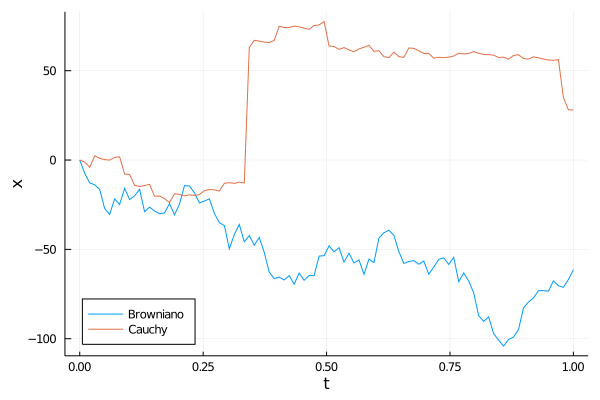
\includegraphics[width=0.4\textwidth]{figures/4_cauchy-brown.png}
    \caption{\scriptsize Processo di Brown e Processo di Cauchy a confronto \href{https://github.com/dodogabrie/Sistemi-Complessi/blob/master/python-project/lezione4/lez4_Cauchy-Brown.ipynb}{Link al codice in Julia}).}
    \label{fig:-fig}
\end{figure}

%%%%%%%%%%%%%%%%%%
%  Chapman form  %
%%%%%%%%%%%%%%%%%%

\subsection{Forma differenziale di Chapman - Kolmogorov}%
\label{sub:Forma differenziale di Chapman - Kolmogorov}
Prendiamo un processo stocastico scomponibile\
\footnote{Ipotesi per cui si può scomporre sul Gardiner}  in una parte continua ed una non continua.\\
Si può dimostrare che un processo di questo tipo è descritto dalla seguente forma differenziale:
\begin{redbox}{Forma di Chapman-Kolmogorov}
    \begin{equation}
    \partial_{t}P(\vect{z},t| \vect{y}, t') = - \Gamma + \Phi
    \label{eq:4_CK}
    \end{equation}
\end{redbox}
\noindent
In cui $\Gamma$ è la parte contenente il processo continuo:
\[\begin{aligned}
    \Gamma = \sum_{i}^{} \partial_{z_i}&\left[ A_i(\vect{z},t) P(\vect{z},t|\vect{y},t') \right] +\\
                         &+\sum_{i,J}^{} \frac{1}{2}\partial^2_{z_iZ_J}\left[ B_{iJ}(z,t) P(\vect{z},t|\vect{y},t') \right]
.\end{aligned}\]
Qui abbiamo un primo termine "deterministico" (con la $A$) che determina soltanto uno spostamento dell'oggetto ed un termine di diffusione (quello in $B$).\\
Nella $\Phi$ abbiamo invece il processo discontinuo:
\[\begin{aligned}
    \Phi = \int  d\vect{x} &\left[\omega (\vect{z}|\vect{x}, t) P(\vect{x},t|\vect{y}, t') \right. + \\
			   & \left. - \omega(\vect{x} | \vect{z}, t)  P(\vect{z},t|\vect{y},t') \right]
.\end{aligned}\]
Il termine $\Phi$ somiglia molto al termine della equazione di Volterra che abbiamo visto nella prima lezione (prob. di trovarsi in $\vect{z}$ è data dalla probabilità di finire in $\vect{z}$ da una posizione $\vect{x}$ diminuito la prob. di scappare in $\vect{x}$ dalla posizione $\vect{z}$).\\
La potenza della equazione è la sua generalità: se sappiamo che un processo è Markoviano (magari per la fisica che ci sta dietro) allora l'equazione di evoluzione delle prob. nel tempo sarà necessariamente quella sopra.
\begin{exmp}[$A=B=0$, quindi $\Gamma =0$]
    \[
        \partial_{t}P = \Phi
    .\] 
    Considerando il rapporto incrementale con passo $\Delta t$:
    \[
	P(z, t+\Delta t|y, t) = P(z,t|y,t) + \Delta t\cdot  \Phi
    .\] 
    Sfruttiamo la proprietà ovvia:
    \[
	P(\vect{z}, t|\vect{t}, t) = \delta (\vect{y}-\vect{z}) 
    .\] 
    Allora possiamo sviluppare l'espressione con $\Delta t$ che tende a $0$ (mettiamoci in una dimensione per semplicità):
    \begin{greenbox}{Soluzione della forma diff. con termini continui}
    \[\begin{aligned}
	P&(z, t + \Delta t| y, t) = \\
				  &= \delta (z-y) \left[1-\Delta t\int dx \omega (x|z) \right] + \Delta t \cdot \omega (z|y) 
    .\end{aligned}\]
    \end{greenbox}
    \noindent
\end{exmp}
\noindent

\subsection{Processo di Wiener}%
\label{sub:Processo di Wiener}
Un processo di Wiener è modellato dalla seguente equazione:
\begin{greenbox}{Equazione per processo di Wiener}
    L'equazione che regola il processo di Wiener è una Fokker-Planck:
    \[
	\frac{\partial }{\partial t} P(\omega,t|\omega_0, t_0) =
	\frac{1}{2}\frac{\partial ^2}{\partial \omega^2} P(\omega, t|\omega_0, t_0) 
    .\] 
\end{greenbox}
\noindent
Inoltre deve esser rispettata la condizione iniziale:
\[
    P(\omega,t_0|\omega_0, t_0) = \delta (\omega-\omega_0) 
.\]
Il processo si può risolvere utilizzando la funzione caratteristica:
\[
    \phi (s, t) = \int d\omega P(\omega, t|\omega_0, t_0) e^{is\omega}
.\] 
Sfruttando le regole della trasformata possiamo riscrivere l'equazione del processo come:
\[
    \frac{\partial \phi }{\partial t} = -\frac{1}{2}s^2\phi
.\] 
\[
    \phi (s, t_0) = \exp (is\omega_0) 
.\] 
La soluzione è nota:
\[\begin{aligned}
    \phi (s) =& \exp\left(-\frac{1}{2}s^2\left(t-t_0\right)\right)\phi (s,t_0)  =\\
    	=&\exp\left(-\frac{1}{2}s^2\left(t-t_0\right) + is\omega_0 \right) 
.\end{aligned}\]
Visto che l'antitrasformata di una Gaussiana è una Gaussiana abbiamo la soluzione nello spazio reale:
\begin{redbox}{Soluzione del processo di Wiener}
    \[
	P(\omega,t|\omega_0, t_0) = 
	\frac{1}{\sqrt{2\pi\left(t-t_0\right)} }
	\exp\left(- \frac{\left(\omega-\omega_0\right)^2}{2\left(t-t_0\right)}\right)
    \] 
\end{redbox}
\noindent
Il processo che abbiamo ottenuto è Gaussiano:
\[
    \left<\omega\right> =  \omega_0
.\] 
\[
    \left<\left(\omega-\omega_0\right)^2\right> = t- t_0
.\] 
\paragraph{Proprietà dei processi di Wiener}%
\label{par:Proprietà dei processi di Wiener}
\begin{itemize}
    \item \'E continuo.
    \item Non è differenziabile, $\forall k$:
	\[\begin{aligned}
	    \text{Prob}&\left(\frac{\left|\omega (t+h) - \omega (t) \right|}{h}> k\right) = \\
		       & = 2 \int_{kh}^{\infty} d\omega  \frac{1}{\sqrt{2\pi  h}} e^{- \omega^2 /2h} 
		       \ \xrightarrow[]{h\to 0} 1
	.\end{aligned}\]
    \item Gli incrementi sono indipendenti:
	\[\begin{aligned}
	    P(&\omega_2, t_2; w_1,t_1; \omega_0,t_0) = \\
	      &= P(\omega_2, t_2|\omega_1,t_1) P(\omega_1, t_1|\omega_0,t_0) P(\omega_0,t_0) 
	.\end{aligned}\]
	Il primo termine dopo l'uguale non dipende da $(\omega_0,t_0)$ perché il processo è Markoviano.
    \item La correlazione: 
    \[
	\left<\omega (t) \omega (s) | \left[\omega_0, t_0\right]\right> = \text{min}(t-t_0, s-s_0) + \omega_0^2
    .\] 
    Che nel caso particolare in cui $\omega_0=t_0=0$ si ha $\left<\omega (t) \omega (s) \right> = s$ se $t>s$.
    \usetikzlibrary{math}
    \tikzmath{\x = 5; \y = 4;}
    \begin{center}
    \begin{tikzpicture}
	 \draw[-stealth] (0,0) --(\x/\y, 0)node[below]{$s$} -- (\x,0) node[right]{$t$};
	 \draw[-stealth] (0,0) --(0,\x/\y)node[left]{$s$} -- (0,\x*2/5) node[above]{$\left<\omega (t) \omega (s) \right>$};
         \draw[thick] 
		  (0,0) node[below]{$0$} -- 
		  (\x/\y,\x/\y)  -- 
		  (\x,\x/\y);
	 \draw[dash dot] 
		  (\x/\y, 0) --
		  (\x/\y, \x/\y);
	\draw[dash dot] 
		  (0,\x/\y) --
		  (\x/\y, \x/\y);

    \end{tikzpicture}
    \end{center}
    \noindent
\end{itemize}
\clearpage

\section{Lezione 5}%
\label{sub:Lezione 5}
\subsection{Processo di Ornstein - Uhlenback}%
\label{sub:Processo di Ornstein - Uhlenback}
Prendiamo in considerazione altri esempi di processi di Markov.
\begin{redbox}{Equazione di Ornstein - Uhlenback}
    \[
	\frac{\partial P}{\partial t} = \frac{\partial }{\partial x} (kxP) + \frac{1}{2}D\frac{\partial ^2}{\partial x^2} P
    .\] 
\end{redbox}
\noindent
\subsubsection{Soluzione stazionaria}%
\label{subsub:Soluzione stazionaria}
Cerchiamo intanto la soluzione con ($\partial_{t}P=0$):
\[
    \frac{\partial }{\partial x} \left(kxP + \frac{1}{2}D \frac{\partial }{\partial x} P\right) = 0 \implies
\] 
\[
    \implies  \left[kxP + \frac{1}{2}D \frac{\partial }{\partial x} P\right]_{-\infty}^{x} = J
.\] 
Se ipotizziamo che:
\[\begin{aligned}
    & 1. \ \lim_{\left|x\right| \to \infty} P(x, t|x_0,t_0) = 0 \\
    & 2. \ \lim_{\left|x\right| \to \infty} xP(x, t|x_0,t_0) = 0
.\end{aligned}\]
Allora possiamo affermare che la corrente $J=0$ per $x\to \infty$. Si risolve allora l'equazione differenziale:
\begin{bluebox}{Soluzione stazionaria}
    \[
    P_s(x) = \frac{1}{\sqrt{\pi} D /k}e^{-kx^2 / D}
    .\] 
\end{bluebox}
\noindent
\subsubsection{Soluzione dipendente dal tempo.}%
\label{subsub:Soluzione dipendente dal tempo}
Per la dipendenza temporale sfruttiamo la funzione caratteristica $\phi (s)$.
\[
    \phi (s) = \int e^{isx}P(x,t|x_0,t_0) dx
.\] 
L'equazione del processo diventa:
\[
    \partial_{t}\phi  = -ks\partial_{s}\phi  - \frac{1}{2}Ds^2\phi
.\] 
Questa equazione alle derivate parziali può essere risolta tramite il metodo delle caratteristiche (\ref{sub:caratteristiche}).\\
L'unico ostacolo all'utilizzo del metodo è il secondo termine dopo l'uguale (contiene la soluzione), vorremmo ricondurci all'equazione in forma standard. \\
Facciamo allora il cambio di variabile:
\[
    g = \ln\phi 
.\] 
Visto che:
\[
     \partial_{t}g =\frac{\partial_{t}\phi}{\phi} \qquad 
     \partial_{s}g = \frac{\partial_{s}\phi}{\phi}
.\] 
Si ha una equazione in $g$ più maneggevole:
\[
    \partial_{t}g + k s \partial_{s}g = -\frac{1}{2}Ds^2
.\] 
Questa è risolubile con il metodo delle caratteristiche: 
\[
    (a, b, c) \to (1, ks, -\frac{1}{2}Ds^2) 
.\] 
Parametrizzando con $\eta$ abbiamo le equazioni caratteristiche:
\[
        \frac{\text{d} t}{\text{d} \eta} = 1 
	\qquad
	\frac{\text{d} s}{\text{d} \eta} = ks 
	\qquad
	\frac{\text{d} g}{\text{d} \eta} = -\frac{1}{2}D s^2
.\] 
Possiamo risolvere per rimuovere $\eta$:
\[
    \begin{cases}
        1. \quad dt = \dfrac{ds}{ks}\\
	2. \quad \dfrac{ds}{ks} = - \dfrac{dg}{1 / 2 Ds^2}
    \end{cases}
\] 
Integrando queste equazioni escono fuori delle costanti, ridefinendo tali costanti come funzioni ($u_1,u_2$) saremo in grado di risalire alla $\phi$.\\ 
Risolviamo la 1:
\[
    c_1 = t - \frac{1}{k}\ln (s) \ \implies  \ c'_1 = \exp\left(t- \frac{1}{k}\ln (s) \right) = s e^{-kt}
.\] 
Quindi definiamo la prima soluzione come $u_1$:
\begin{equation}
    u_1(t,s) = s e^{-kt} \label{eq:cat1}
\end{equation}
Passiamo alla equazione 2 del sistema, integrando si ottiene:
\[
    c_2 = \frac{s^2D}{4k} + g 
.\] 
Ricordando che $g=\ln\phi$ possiamo definire anche un'altra funzione a partire dalla costante $c_2$ (si fa l'esponenziale della 2):
\begin{equation}
    u_2(t,s) = \phi \exp\left(\frac{Ds^2}{4k}\right) \label{eq:cat2}
\end{equation}
Riscrivendo la \ref{eq:cat2} isolando $\phi$ si ha:
\[
    \phi  = u_2 \exp\left(-\frac{Ds^2}{4k}\right)
.\]
Visto che $u_1$ e $u_2$ sono entrambe costanti collegate dalle equazioni caratteristiche sarà vero che:
\[
    u_2 = f(u_1) 
.\] 
\begin{redbox}{Soluzione dipendente dal tempo per $\phi$}
    \begin{equation}
    \phi =f\left(se^{-kt}\right)\exp\left(-\frac{Ds^2}{4k}\right) 
    \label{eq:car_phi}
    \end{equation}
\end{redbox}
\noindent
\subsubsection{Condizioni al contorno}%
\label{subsub:Condizioni al contorno}
\[
    P(x,0|x_0,0) = \delta (x-x_0) \implies  \phi (s,0) = e^{ix_0s}
.\] 
Prendiamo l'equazione \ref{eq:car_phi} ed invertiamola per trovare la $f(s)$ ($t=0$) inserendo anche la condizione iniziale:
\[
	f(s) = e^{ix_0s}\exp\left(\frac{Ds^2}{4k}\right)
.\] 
Per reinserire il tempo e trovare la soluzione con queste condizioni iniziali basta fare la sostituzione:
\[
    s \to se^{-kt}
.\] 
\begin{redbox}{Soluzione con condizione iniziale $\delta$}
    \begin{equation}
	\phi(s,t) =
	\exp\left[-\frac{Ds^2}{4k}\left(1-e^{-2kt}\right) + isx_0e^{-kt}\right]
    \end{equation}
\end{redbox}
\noindent
A questo punto possiamo tornare indietro con una antitrasformata, altrimenti possiamo ricavare i momenti sfruttando le proprietà di $\phi$:
\[
    \left<x(t)\right> = \left.i\frac{\partial \phi}{\partial s} \right|_{s=0} = x_0e^{-kt}
.\] 
\[\begin{aligned}
    \text{var(x(t) )} =& \left<x^2(t)\right> - \left<x(t)\right>^2 = \\
    =& \left.-1 \frac{\partial ^2\phi}{\partial s^2}\right|_{s=0} - \left<x\right>^2 = \\
    =&\frac{D}{2k}\left(1-e^{-2kt}\right)
.\end{aligned}\]

\begin{figure}[H]
    \centering
    \begin{tikzpicture}
	\begin{axis}[
	    xmin= 0, xmax= 4,
	    ymin= 0, ymax = 1.2,
	    axis lines = middle,
	    xlabel={t},
	    ylabel={},
	    ytick={0.5, 1},
	    yticklabels={$\frac{D}{2k}$, $x_0$ },
	    xtick={0},
	    xticklabel={$$},
	]
	\addplot[domain=0:4, samples=100, color=red]{e^(-x)};
	\addlegendentry{$\left<x(t) \right>$ }
	\addplot[domain=0:4, samples=100, color=blue]{1/2*(1-e^(-2*x) ) };
	\addlegendentry{var($x(t)$) }
	\addplot[dotted, domain=0:4, samples=100]{0.5};
	\end{axis}
    \end{tikzpicture}
    \caption{\scriptsize Andamento della media e della varianza per il processo di Ornstein-Uhlenback.}
    \label{fig:mean-var}
\end{figure}
\noindent
I risultati ottenuti sono conformi con le condizioni iniziali inserite. 
\paragraph{Media}%
all'istante iniziale tutti i camminatori sono in $x_0$ (grazie alla $\delta$). \\
Quando il processo fa evolvere le posizioni dei camminatori allora i camminatori si allontanano da $x_0$ andando verso l'origine, questo è conforme con quanto visto per la soluzione stazionaria: una Gaussiana centrata nello $0$.
\paragraph{Varianza}%
Nell'istante iniziale, quando tutti i camminatori sono nel punto $x_0$, la varianza è nulla, questa si stabilizza nel tempo al valore dato dalla Gaussiana nelle condizioni stazionarie.
\subsubsection{Calcolo delle correlazioni}%
\label{subsub:Calcolo delle correlazioni}
\[\begin{aligned}
    \left<x(t_1) x(t_2) \right.&\left.|\left[x_0,t_0\right]\right> =\\
    =&\int dx_1dx_2 P(x_1,t_1;x_2,t_2;x_0,t_0) x_1x_2 = \\
    =&\int dx_1dx_2 x_1x_2P(\overline{x}_1,\overline{x}_2) P(\overline{x}_2, \overline{x}_0) 
.\end{aligned}\]
In cui si è assunto il processo Markoviano e la gerarchia temporale: $t_1>t_2>t_0$.\\
Se il processo ha raggiunto la stazionarietà ($t_0\to \infty$) allora conosciamo la forma del propagatore:
\[
    P(x_2|x_0) \sim \exp\left(-k \frac{x_2^2}{D}\right)
.\] 
Risolvendo con questa si ottiene:
\begin{redbox}{Correlazione temporale a due}
    \[
	\left<x(t) x(s) \right> \sim \frac{D}{2k}\exp\left(-k\left|t-s\right|\right)
    .\] 
    La correlazione temporale delle posizioni decade esponenzialmente.
\end{redbox}
\noindent

\subsubsection{Ornstein-Uhlenback come modello per rumore realistico.}%
\label{subsub:Ornstein-Uhlenback come modello per rumore realistico.}
Facendo la trasformata di Fourier della funzione di Correlazione si ottiene una Lorenziana:
\[\begin{aligned}
    S_{OU}(\omega) = & \mathcal{F}\left(\left<x(t) x(s) \right>\right)=\\
		     =&\frac{1}{\omega^2 /k ^2 + 1}
.\end{aligned}\]

\begin{figure}[H]
    \centering
    \begin{tikzpicture}
	\begin{axis}[
	    xmin= 0, xmax= 4,
	    ymin= 0, ymax = 1.5,
	    axis lines = middle,
	    xlabel={$\omega$},
	    ylabel={$S_{OU}(\omega)$},
	    ytick={1, 0.5},
	    yticklabels={$S_{OU}(0)$, $S_{OU}(0)/2$ },
	    xtick={0, 1},
	    xticklabels={$$ ,$\sim k$},
	    every axis x label/.style={
		at={(axis description cs:1,-0.1)},
		anchor=south,
                },
	]
	\addplot[domain=0:4, samples=100, color=red]{1/(x^2 + 1) };
	\addplot[dotted, domain=0:1, samples=100]{0.5};
	\addplot[dotted, domain=0:1, samples=100] coordinates{(1,0)(1,0.5)};
	\end{axis}
    \end{tikzpicture}
    \caption{\scriptsize Andamento della trasformata della correlazione per il processo di Ornstein-Uhlenback.}
    \label{fig:mean-var}
\end{figure}
\noindent
Questo è esattamente quello che ci aspettiamo da un rumore realistico: il rumore ha una frequenza di cut-off dettata da una Lorenziana.	\\
Il cut-off è dovuto al fatto che le cose non possono muoversi infinitamente veloci, l'inerzia dei corpi che partecipano al moto stocastico fissa la frequenza di cut-off.\\
C'è quindi un tempo caratteristico di osservazione del fenomeno
\[
    \tau  = \frac{1}{k}
.\] 
Se osserviamo il moto su scale temporali di quest'ordine allora lo spettro degli urti tra i corpi va a zero, questo comporta che il moto oltre queste scale temporali non è più ben descritto dal processo di Wiener.
\begin{ex}{Modifica all'equazione di OU}
    Risolvere l'equazione di Ornstein-Uhlenback con l'aggiunta di un termine nella $\partial_{x}$:
    \[
	\frac{\partial P}{\partial t} = \frac{\partial }{\partial x} (\left(kx + \alpha\right)P) + \frac{1}{2}D\frac{\partial ^2}{\partial x^2} P
    .\] 
    \textbf{Soluzione}: Il moto dovrebbe andare a stazionarietà nel punto $-\alpha  / k$.
\end{ex}
% Appendice
%%%%%%%%%%%%%%%%%%%%%%%%%%
%  Codice per appendice  %
%%%%%%%%%%%%%%%%%%%%%%%%%%
\noindent\rule{0.48\textwidth}{0.7pt}
\newpage
\addtocounter{Sec}{\value{section}}%Mantengo il numero delle sezioni
\begin{appendices}
\section*{Appendice}%
\setcounter{section}{\theSec}%Applico numero sezioni
\setcounter{subsection}{0}%Applico numero sezioni
\renewcommand{\thesubsection}{\arabic{section}.\Alph{subsection}}

\subsection{Metodo delle Caratteristiche.}
\label{sub:caratteristiche}
Supponiamo di avere una PDE della forma:
\begin{redbox}{PDE per metodo delle caratteristiche}
\[
    a(x,y) \partial_{x}u + b(x,y) \partial_{y}u - c(x, y) = 0
.\] 
\end{redbox}
\noindent
Scrivibile anche come:
\begin{equation}
    \left(a,\ b,\ c\right)\cdot \left(\partial_{x}u,\ \partial_{y}u,\ -1\right) = 0
    \label{eq:caratt}
\end{equation}
Ed una superficie parametrizzata con la soluzione della PDE ($u(x,y))$: 
\[
    S \equiv (x,y, u(x,y) ) 
.\] 
%\begin{center}
\begin{tikzpicture}[x={(170:.9cm)},y={(55:.6cm)},z={(90:1cm)}]
  %%%%%%%%%%%%%%%%%%%%
  %  Piano Tangente  %
  %%%%%%%%%%%%%%%%%%%%
  \tikzmath{\x = 2.2; \z = -0.4;}
  %%%%%%%%%%%%%%%%%
  %  Piano curvo  %
  %%%%%%%%%%%%%%%%%
  \draw[fill=red!75!black, opacity=0.5, looseness=.8] (\x,-\x,\z) node[above right] {$S$}
  to[bend left] (\x,\x,\z)
  to[bend left] coordinate (mp) (-\x,\x,\z)
  to[bend right] (-\x,-\x,\z)
  to[bend right] coordinate (mm) (\x,-\x,\z)
  -- cycle;
  %%%%%%%%%%
  %  Assi  %
  %%%%%%%%%%
  \draw[->] (0.5,0,-1.5) -- (-3,0,-1.5) node[right] {$y$};
  \draw[->] (0,0.4,-1.5) -- (0,-3,-1.5) node[right] {$x$};
  \draw[->] (0,0,-2) -- (0,0,1.5) node[right] {$u(x,y)$};
\end{tikzpicture}
\end{center}

\noindent
\subsubsection{Vettore tangente a $S$}%
\label{subsub:Vettore tangente a S}
\begin{bluebox}{}
Il vettore $\left(a, \ b, \ c\right)$ appartiene al piano tangente di $S$ in ogni punto $\left(x, y, z\right)$.
\end{bluebox}
\noindent
La normale $\vect{N}$ alla superficie $S$ la si trova facendo il gradiente di:
\[
    \overline{S} = u(x,y) - z
.\] 
Si ottiene quindi:
\[
    \vect{N}  = \left(\partial_{x}u, \ \partial_{y}u, \ -1\right)
.\] 
Visto che $\vect{N}$ è il secondo termine nella \ref{eq:caratt} si vede che la soluzione è il luogo dei vettori $(a, b,c)$ ortogonali a $\vect{N}$, quindi tangenti al piano $S$.
%\begin{center}
\begin{tikzpicture}[x={(170:.9cm)},y={(55:.6cm)},z={(90:1cm)}]
  %%%%%%%%%%%%%%%%%%%%
  %  Piano Tangente  %
  %%%%%%%%%%%%%%%%%%%%
  \tikzmath{\x = 2.; \z = 0;}
  \draw[fill=black, opacity=0.3] (\x,-\x,\z) -- (\x,\x,\z) -- (-\x,\x,-\z) -- (-\x,-\x,-\z) -- cycle;
  %%%%%%%%%%%%%%%%%
  %  Piano curvo  %
  %%%%%%%%%%%%%%%%%
  \draw[fill=red!75!black, opacity=0.5, looseness=.8] (2.5,-2.5,-1) node[above right] {$S$}
  to[bend left] (2.5,2.5,-1)
  to[bend left] coordinate (mp) (-2.5,2.5,-1)
  to[bend right] (-2.5,-2.5,-1)
  to[bend right] coordinate (mm) (2.5,-2.5,-1)
  -- cycle;
  %%%%%%%%%%
  %  Assi  %
  %%%%%%%%%%
  \draw[->] (0,0,0) -- (0,-2.7,0) node[right] {$(a, b, c) $};
  \draw[->] (0,0,0) -- (0,0,2) node[right] {$N$};
\end{tikzpicture}
\end{center}

\noindent
Quindi la soluzione della PDE è tale per cui il vettore $(a,b,c)$ sta sul piano tangente.

\subsubsection{Curva caratteristica}%
\label{subsub:Curva caratteristica}
Per mappare la soluzione si introduce una curva $C$ detta curva caratteristica che descrive la superficie. 
\[
    C: \quad C \equiv \left(x(\eta) , y(\eta), z(\eta) \right)
.\] 
$C$ è una curva parametrica in $\eta$ localmente tangente a $(a, b, c)$.\\
La condizione di parallelismo implica il seguente sistema:
\begin{greenbox}{Equazioni Caratteristiche}
    Sono curve integrali per il campo vettoriale $(a, b, c)$ 
\[
    \begin{cases}
	 &a(x(\eta) , y(\eta) ) = \dfrac{\text{d} x}{\text{d} \eta} \\
								   &\\
	 &b(x(\eta) , y(\eta) ) = \dfrac{\text{d} y}{\text{d} \eta} \\ 
								   &\\
	 &c(x(\eta) , y(\eta) ) = \dfrac{\text{d} z}{\text{d} \eta}  
    \end{cases}
\]
\end{greenbox}
\noindent
Queste equazioni risolvono la PDE.
\begin{exmp}[Equazione del trasporto.]
   \[
       u_t + a \cdot u_x = 0
   .\]  
   In questo caso si ha $(a, b, c) \to (a, 1, 0)$, quindi:
   \[\begin{aligned}
	   &\dfrac{\text{d} x}{\text{d} \eta} = a & \quad
	   &\dfrac{\text{d} t}{\text{d} \eta} = 1 & \quad
	   &\dfrac{\text{d} z}{\text{d} \eta} = 0 &
   \end{aligned}\]
   Passiamo alla risoluzione:
   \[
       \begin{cases}
	    x(\eta) = a\eta +c_1\\
	    t(\eta) = c_2 + \eta\\
	    z(\eta) = c_3
       \end{cases}
       \implies\quad
       \begin{cases}
           x -at = x_0\\
	   z=k
       \end{cases}
   \] 
   In cui si è effettuata dell'algebra per eliminare $\eta$ nel primo sistema. 
   \begin{itemize}
       \item La funzione che risolve il sistema di destra è la soluzione dell'equazione del trasporto. 
       \item  Graficamente le funzioni che risolvono sono delle rette con $z$ costante, l'unione di queste rette rappresenta $S$.
       \item Abbiamo ottenuto un fascio di soluzioni poiché non abbiamo imposto alcuna soluzione al contorno.
   \end{itemize}
   In conclusione $z$ dovrà essere funzione di $x-at$, quindi la soluzione generale sarà una funzione del tipo:
   \[
       z(x, t ) = f(x-at) \equiv u(x, t) 
   .\] 
   Supponiamo che all'istante iniziale la soluzione fosse una gaussiana:
   \[
       f(x, t=0) = e^{-x^2}
   .\] 
   Quindi si ha che anche la soluzione a $t=0$ è una gaussiana:
   \[
       u(x, t=0) = e^{-x^2}
   .\] 
   Ed introducendo il tempo la soluzione diventa semplicemente:
   \[
       u(x, t) = e^{-\left(x-at\right)^2}
   .\] 
   
\end{exmp}
\noindent

\end{appendices}

\renewcommand{\thesubsection}{\arabic{section}.\arabic{subsection}}
%%%%%%%%%%%%%%%%%%%%%%%%%


\clearpage

\section{Lezione 6}%
\label{sub:Lezione 6}

\subsection{Modelli semplici di Random Walk}%
\label{sub:Random Walk}

Mettiamoci in una situazione unidimensionale, con un oggetto che può fare salti di ampiezza unitaria.
\usetikzlibrary{arrows.meta,bending}
\begin{center}
\begin{tikzpicture}[bullet/.style={circle,inner sep=0.7ex},x=2cm,auto,bend angle=40]
    \tikzmath{\x = 1.5; \z = 0;}
    \draw[->] (-\x,0) -- (\x,0) node[below right]{$x$};
    \path (-\x/3,0) node[bullet] (-a) {}
     (0,0) node[bullet] (0) {}
     (\x/3,0) node[bullet] (a) {};
    \foreach \Y [count=\X starting from -2] in {-2,-1,0,1,2} 
     {\draw (\X/2,0.05) -- (\X/2,-0.1) node[below]{$\Y$};}
    \draw[-{Stealth[bend]},thick] (0) to[bend left] node{$+1$} (a);
    \draw[-{Stealth[bend]},thick] (0) to[bend right] node[above]{$-1$} (-a);
\end{tikzpicture}
\end{center}

Possiamo analizzare due modelli di RW:
\begin{enumerate}
    \item Salto di $\pm 1$ ad un tempo casuale.
    \item Salto di $\pm 1$ ad un tempo $\tau$ fissato.
\end{enumerate}
Entrambi i casi descrivono processi Markoviani.
\subsubsection{1. Salto ad un tempo random.}%
\label{subsub:1. Salto ad un tempo random.}
L'equazione di Chapman-Kolmogorov in forma differenziale per il processo si scrive come:
\[\begin{aligned}
    \partial_{t}P\left(n,t|n',t'\right) = \left[ \ \right.&\omega\left(n|n+1,t\right)P\left(n+1, t|n',t'\right) +\\
                                             +& \omega\left(n|n-1,t\right)P\left(n-1, t|n',t'\right) + \\
					     -& \left. 2P\left(n,t|n',t'\right) \ \right]
.\end{aligned}\]
Facciamo chiarezza sui termini in equazione, prendiamo il primo nella parentesi quadra dopo l'uguale:
\[
    \omega\left(n|n+1,t\right)P\left(n+1, t|n',t'\right)
.\] 
Questo indica la probabilità di essere in $n+1$ (descritta dal termine $P$) e di fare un salto all'indietro (descritta dalla probabilità corrispondente $\omega$).\\
L'ultimo termine in parentesi indica la probabilità di essere in $n$ al tempo $t$, se ci troviamo in tal punto allora allo step successivo usciamo sicuramente fuori per costruzione del moto.\\
Imponendo che il rate di salto in avanti sia uguale a quello di salto all'indietro:
\begin{equation}
    \omega (n+1|n,t) = \omega (n-1|n,t) \equiv d \label{6_rate}
\end{equation}
Possiamo semplificare l'equazione del processo:
\begin{bluebox}{Chapman-Kolmogorov per RW 1.}
    \begin{equation}
\begin{aligned}
    \partial_{t}P\left(n,t|n',t'\right) = d\left[ \ \right.&P\left(n+1, t|n',t'\right) +\\
                                             +& P\left(n-1, t|n',t'\right) + \\
					     -& \left. 2P\left(n,t|n',t'\right) \ \right]
					     \label{eq:RW_1}
.\end{aligned}
    \end{equation}
\end{bluebox}
\noindent
Si risolve in trasformata:
\[
    G(s,t) = \left<e^{isn}\right> = \sum_{n}^{\infty} P\left(n,t|n',t'\right)e^{isn}
.\] 
Quando abbiamo un termine del tipo $P\left(n\pm 1|n',t'\right)$ basta scrivere:
\[
    e^{isn}P\left(n\pm 1, t|n',t'\right) = e^{\mp is} e^{is(n\pm 1)}P\left(n\pm 1, t|n',t'\right)
.\] 
Quindi inserendo nella equazione di CK:
\[
    \partial_{t}G(s,t) =d\left(e^{-is}+ e^{is}-2\right)G(s,t) 
.\] 
Si risolve per $G(s,t)$:
\[
    G(s,t) = \exp \left[\left(e^{is}+e^{-is}-2\right)td\right]G(s,0) 
.\] 
Andando a cercare la soluzione stazionaria si ha che:
\[
t\to \infty \implies s\to 0
.\] 
Questo per le relazioni tra spazio reale e trasformata: in sostanza stiamo assumendo i camminatori come oggetti reali, quindi se $\omega\to 0$ dev'essere necessariamente che $s\to 0$:
\[
    \omega  \sim sc
.\] 
Tornando alla $G$ sviluppando si ottiene una Gaussiana:
\[
    G(s,t) = \exp(-s^2td) 
.\] 

\subsubsection{2. Salto ad un tempo $\tau$ fissato}%
\label{subsub:2. Salto ad un tempo tau fissato}
In questo caso il tempo è una variabile discreta di passo $\tau$.
\begin{bluebox}{Equazione per il propagatore nel RW 2}
\begin{equation}
\begin{aligned}
    P\left(n,(N+1) \tau|\right.&\left.n',N'\tau\right)= \\
			       &\frac{1}{2}\left[P\left(n+1,N\tau|n',N'\tau\right)\right. + \\
			       & \quad + \left.  P\left(n-1,N\tau|n',N'\tau\right)\right] \label{eq:6_1}
.\end{aligned}
\end{equation}
    
\end{bluebox}
\noindent

\begin{greenbox}{RW1 e RW2 equivalenti per scale piccole.}
 Se $\tau$ è piccolo rispetto a $N\tau$ il caso (2) diventa equivalente al caso (1).   
\end{greenbox}
\noindent
Definiamo il tempo $t' = N'\tau$:
\begin{equation}
\begin{aligned}
    P\left(n,(N+1) \tau|n',N'\tau\right)\simeq & P\left(n,N\tau|n',t'\right) + \\
					       & + \tau\partial_{t}P\left(n,N\tau|n',t'\right) \label{eq:6_2}
.\end{aligned}
\end{equation}
Si procede definendo: 
\[
 d \equiv 1 /2\tau   
.\] 
Possiamo ottenere l'equazione \ref{eq:RW_1} sostituendo al primo termine della \ref{eq:6_1} il secondo della \ref{eq:6_2} .\\
Risolviamo adesso la \ref{eq:6_1} con il metodo della funzione caratteristica ($G(s,t) = \left<e^{ins}\right>$ ):
\[
    G(s, (N+1)\tau) = \frac{1}{2}\left(e^{is}+ e^{-is}\right)G(s,N\tau) 
.\] 
Come condizione iniziale si impone che $G(s,0) = 1$.\\
In questo modo l'equazione in $G$ è una ricorsiva in $N$ che ha soluzione:
\[
    G(s,N\tau) = \left(\frac{1}{2}\left(e^{is}+e^{-is}\right)\right)^{N}
.\] 
A questo punto possiamo vedere che se $N\to \infty$ si ottiene una soluzione Gaussiana come nell'RW1 (mandare $N\to \infty$ significa limite stazionario).
\[
    \begin{cases}
        \tau N = t\\
	d = \dfrac{1}{2\tau}
    \end{cases}
    \implies  
    \frac{td}{N} = \frac{1}{2}
.\] 
\[
    G(s,N\tau) = \left[1 + \frac{td}{N}\left(e^{is}+ e^{-is}-2\right)\right]^N
.\] 
Sfruttando il limite notevole:
\[
    \lim_{x \to \infty} \left(1+\frac{\alpha}{x}\right)^{x} = e^{\alpha}
.\] 
Si ottiene:
\[
    G(s, N\tau) \xrightarrow[]{N \to \infty} G(s,t) = \exp\left[td\left(e^{is}+e^{-is}-2\right)\right]
.\] 
In conclusione è come se, aspettando abbastanza a lungo, la caoticità sul salto di $\pm 1$ contagiasse il clock di salto $\tau$ rendendo anch'esso caotico come nel caso RW1.\\
Nel proseguo distingueremo i due casi solo dove necessario vista la loro equivalenza a stazionarietà.

\subsubsection{Limite al continuo nei salti}%
\label{subsub:Limite al continuo}
Definiamo lo spazio percorso dal camminatore dopo $n$ step in un reticolo di passo $l$:
\[
    x = nl
.\] 
\usetikzlibrary{arrows.meta,bending}
\begin{center}
\begin{tikzpicture}[bullet/.style={circle,inner sep=0.7ex},x=2cm,auto,bend angle=40]
    \tikzmath{\x = 1.5; \z = 0;}
    \draw[->] (-\x,0) -- (\x,0) node[below right]{$x'$};
    \path (-\x/3,0) node[bullet] (-a) {}
     (0,0) node[bullet] (0) {}
     (\x/3,0) node[bullet] (a) {};
    \foreach \Y [count=\X starting from -2] in {-2l,-l,0,l,2l} 
     {\draw (\X/2,0.05) -- (\X/2,-0.1) node[below]{$\Y$};}
    \draw[-{Stealth[bend]},thick] (0) to[bend left] node{$+l$} (a);
    \draw[-{Stealth[bend]},thick] (0) to[bend right] node[above]{$-l$} (-a);
\end{tikzpicture}
\end{center}

Quello che faremo sarà far il limite per $l\to 0$.\\
La trasformata si modifica per questo caso nel seguente modo:
\begin{equation}
\begin{aligned}
    \phi (s,t) = &\left<e^{isx}\right> = G(ls, t) =\\
		 & = \exp \left[\left(e^{ils} + e^{-ils} -2 \right)td\right]
		 \label{eq:6_continuo}
.\end{aligned}
\end{equation}
Dove ricordiamo che $d$ è il rate del processo definito dalla \ref{6_rate}.\\
Si studia adesso anche il caso stazionario, quindi dobbiamo effettuare entrambi i limiti:
\[\begin{aligned}
    &l\to 0\\
    &\tau\to 0
.\end{aligned}\]
Sviluppando nell'esponenziale della \ref{eq:6_continuo} ci si rende conto che sopravvive solo il termine:
\[
    \sim \exp\left(-s^2l^2td\right)
.\] 
Per questo è necessario che:
\[
    D = \lim \limits_{\substack{%
	         l \to 0\\
		  d \to \infty}} l^2d = \text{Finito}
.\] 
Fare il limite per il Rate $d\to \infty$ è lo stesso che fare il limite per $\tau\to 0$ poiché per definizione $d = 1 /2\tau$.\\
In conclusione otteniamo un andamento per $\phi$ Gaussiano:
\begin{bluebox}{Funzione caratteristica per RW nel limite continuo}
\[
    \phi (s,t) = \exp\left(-s^2tD\right)
.\]     
\end{bluebox}
\noindent
Quindi abbiamo anche che:
\begin{equation}
    \left<x^2\right> \sim  2tD \label{eq:6_mom_sec}
\end{equation}
\subsubsection{Random Walk e processi di Wiener}%
\label{subsub:Random Walk e processi di Wiener}
Si può dimostrare che per $l\to 0$ l'equazione che regola il propagatore $P$ è una Fokker-Plank (che regola anche i processi di Wiener). \\
Partiamo dalla Master Equation già scritta sopra:
\[\begin{aligned}
    \partial_{t}P(n) = d\left(P(n+1) + P(n-1) -2 P(n) \right)
.\end{aligned}\]
Sviluppando in $l=0$ si ha:
\[\begin{aligned}
    &P(n+1) = P(n) + \partial_{x}P(n) l + \frac{1}{2}\partial^2_{x^2} l^2P(n) \\
    &P(n+1) = P(n) - \partial_{x}P(n) l + \frac{1}{2}\partial^2_{x^2} l^2P(n)
.\end{aligned}\]
E reinserendo nella equazione per $P$ si ha:
\[
    \partial_{t}P(n) = dl^2 \partial^2_{x^2} P(n) 
.\] 
Che è appunto una Fokker-Plank.

\subsection{Random Walk di Weierstrass}%
\label{sub:Random Walk di Weierstrass}
Questo RW è più complesso dei primi due, si basa su alcuni parametri che ne determinano il passo ed il rate: ($N$, $b$).\\
Adesso anziché fare salti fissi di $l$ si fanno salti $J_n$ con rate $R_n$ che variano al variare dell'intero $n$. $J_n$ e $R_n$ sono così definiti:
\[
    J_n = \left(N^{n}+1\right)l \qquad R_n = \frac{\gamma}{b^n} \qquad b,N > 1
.\] 
\[
    n \in \left[0\ldots\infty\right]
.\] 
\usetikzlibrary{arrows.meta,bending}
\begin{center}
\begin{tikzpicture}[bullet/.style={circle,inner sep=0.7ex},x=2cm,auto,bend angle=40]
    \tikzmath{\x = 1.5; \z =3.; \w = 0.5;}
    \draw[->] (-\w,0) -- (\z,0) node[below right]{$x$};
    \path 
	(-\w,0) node[bullet] (-a) {}
        (0,0) node[bullet] (0) {}
        (\w,0) node[bullet] (a) {};
    \foreach \X\Y in {-\w/-l, 0/0, \w/l, 2*\w/\left(N+1\right)l , 5*\w/\left(N^2+1\right)l}
    { \draw (\X,0.05) -- (\X,-0.1) node[below]{$\Y$};}
    \draw[-{Stealth[bend]},thick] (0) to[bend right=20]node[above]{$-R_0$ } (-a);
    \draw[-{Stealth[bend]},thick] (0) to[bend left=20] node[above]{$R_0$ } (a);
    \draw[-{Stealth[bend]},thick] (0) to[bend left=90] node[above]{$R_1$} (2*\w,0);
    \draw[-{Stealth[bend]},thick] (0) to[bend left=90] node[above]{$R_2$ } (5*\w,0);
\end{tikzpicture}
\end{center}

Possiamo considerare $\gamma$ come il parametro corrispondente a $d$ della sezione precedente.
Quindi ad esempio si può avere:
\begin{itemize}
    \item Salto di $l$ con rate $\gamma$. 
    \item Salto di $\left(N+1\right)l$ con rate $\gamma  / b$.
    \item Salto di $\left(N^2+1\right)l$ con rate $\gamma /b^2$.
\end{itemize}
Come conseguenza salti più lunghi avranno rate più bassi (quindi saranno meno frequenti).\\
\subsubsection{Master Equation per il RW di Weierstrass}%
\label{subsub:Master Equation per il RW di Weierstrass}
\[\begin{aligned}
    \partial_{t}P\left(n,t|n',t'\right) = &\sum_{i=0}^{\infty} 
    \frac{\gamma}{b^{i}} \left[P\left(n+(N^{i}+1) ,t|n',t'\right) \right. + \\
		    & \qquad \quad + \left. P\left(n-(N^{i}+1) ,t|n',t'\right)\right] + \\
		     - &2 \sum_{i=0}^{\infty} \left(\frac{1}{b^{i}}\right) P\left(n,t|n',t'\right)
.\end{aligned}\]
La prima sommatoria tiene di conto di tutti i punti che possono arrivare da distanze diverse. La seconda sommatoria invece tiene conto di quelli che sono già nel punto e scappano via.\\
L'equazione descrive un processo a salti, di conseguenza il moto in questione è Markoviano. Come per gli altri RW risolviamo con la funzione caratteristica.
\[
    G(s,t) = \left<e^{isn}\right> = \sum_{n}^{\infty} e^{isn}P(n,t|n',t') 
.\] 
La master equation si riscrive come:
\[\begin{aligned}
    \partial_{t}G(s,t) = \gamma &\left[e^{is}\left( 1 + \sum_{n=0}^{\infty} \frac{e^{isN^{n}}}{b^{n}} \right) + \right.\\  
				& \ \ \left. + e^{-is}\left( 1 + \sum_{n=0}^{\infty} \frac{e^{-isN^{n}}}{b^{n}} \right) + \right.\\
				& \qquad \qquad \qquad \qquad \ \left.- 2 \sum_{n=0}^{\infty} \frac{1}{b^n} \right]G(s,t) 
.\end{aligned}\]
Possiamo compattare la scrittura con la notazione:
\[
    f(s) \equiv \left[e^{is}\left( 1 + \sum_{n=0}^{\infty} \frac{e^{isN^{n}}}{b^{n}} \right) + C.C - 2 \sum_{n=0}^{\infty} \frac{1}{b^n} \right]
.\] 
Che ci permette di esprimere direttamente il risultato:
\begin{bluebox}{Funzione caratteristica per il RW di Weierstrass}
\[
    G(s,t) = \exp\left(tf(s)\right)G(s,0) 
.\]     
\end{bluebox}
\noindent
\subsubsection{Limite stazionario}%
\label{subsub:Limite stazionario}
Vediamo se anche in questo caso mandando $t\to \infty$ si ottiene una Gaussiana come nei casi RW1 e RW2.\\
Sviluppando la $G$ per $s\to 0$ si ottiene che molti termini polinomiali si ammazzano a vicenda, rimane soltanto la seguente:
\[
    G(s,t) = \exp\left(-ts^2 \sum_{k=0}^{\infty} \left(\frac{N^2}{b}\right)^k\right)
.\] 
All'esponente notiamo che il coefficiente di diffusione $D$ è una sommatoria:
\[
    D \to \sum_{k=0}^{\infty} \left(\frac{N^2}{b}\right)^k\
.\] 
Quello che si scopre è quindi che il parametro $N^2 /b$ decide se il processo sarà Gaussiano o no, infatti:
\begin{redbox}{}
\begin{itemize}
    \item Se $N^2 /b< 1$ abbiamo una serie geometrica all'esponenziale che ci riconduce ad una forma Gaussiana.
    \item Se $N^2 /b > 1$ la sommatoria diverge, il processo resta Markoviano ma non vale più il teorema del limite centrale.
\end{itemize}
\end{redbox}
\noindent
Visto che il momento secondo è proporzionale a $D$ (eq. \ref{eq:6_mom_sec}) se ne conclude un processo con $N^2 /b > 1$ ha varianza infinita.\\
La cosa interessante è che abbiamo scoperto un processo random che al limite non diventa una Gaussiana \footnote{il momento secondo deve essere definito nelle ipotesi per il teorema del limite centrale\ldots}

\subsection{Random Telegraph}%
\label{sub:Random Telegraph}
Il RT è un processo random che coinvolge un sistema a due stati (o livelli):
\usetikzlibrary{math}
\tikzmath{\x = 5; \y = 0.5; \Y = 2;}
\begin{center}
\begin{tikzpicture}
     \draw[-stealth] (0,0) node[below]{$0$}-- (\x,0) node[right]{$t$};
     \draw[-stealth] (0,0) -- (0,\y)node[left]{$b$} -- (0,3*\y)node[left]{$a$} -- (0,\Y) node[above]{$RT$};
     \draw[thick] (0,\y) -- 
		  (1,\y);
     \draw[dotted](1,\y) --  
                  (1, 3*\y);

     \draw[thick] (1,3*\y) -- 
		  (2,3*\y);
     \draw[dotted](2,3*\y) --  
                  (2, \y);

     \draw[thick] (2,\y) -- 
		  (2.5,\y);
     \draw[dotted](2.5,\y) --  
                  (2.5,3*\y);

     \draw[thick] (2.5,3*\y) -- 
		  (4,3*\y);
     \draw[dotted](4,3*\y) --  
                  (4,\y);

     \draw[thick] (4,\y) -- 
		  (5,\y);

\end{tikzpicture}
\end{center}
\noindent

Il processo è descritto dalle equazioni differenziali:
\[\begin{aligned}
    &\partial_{t}P\left(a,t|x,t_0\right) = -\lambda P\left(a,t|x,t_0\right) + \mu P\left(b,t|x,t_0\right)\\
    &\partial_{t}P\left(b,t|x,t_0\right) = \lambda P\left(a,t|x,t_0\right) - \mu P\left(b,t|x,t_0\right)
.\end{aligned}\]
In cui $x$ può essere $a$ oppure $b$.\\
In questo caso c'è anche una terza equazione per la normalizzazione del processo:
\[
    P\left(a,t|x,t_0\right)+ P\left(b,t|x,t_0\right) = 1
.\] 
Si scelgono le condizioni iniziali:
\[
    P\left(x,t_0|x',t_0\right) = \delta_{xx'}
.\] 
E quello che si ottiene risolvendo le equazioni differenziali è:
\begin{equation}
    P\left(x', t|x,t_0\right) =  \frac{\omega (x') }{R} + e^{-R (t-t_0)}\left(\frac{\lambda}{R}\delta_{ax} + \frac{\mu}{R}\delta_{bx}\right)
    \label{eq:6_RT}
\end{equation}
In cui $R$ è la somma dei due rate:
\[
    R = \mu +\lambda
.\] 
Mentre la funzione $\omega (x')$ differenzia i casi con $x'=a$ e $x'=b$:
\[
    \omega(x') =
    \begin{cases}
        \lambda  \quad \text{ se } x' = a\\
        \mu  \quad \text{ se } x' = b
    \end{cases}
.\]
Il primo termine nella \ref{eq:6_RT} è il termine stazionario. Il secondo termine invece decade esponenzialmente in $t$, il termine con le  $\delta$  a moltiplicare deriva dalle condizioni iniziali inserite.
\[\begin{aligned}
    \left<x(t) | \left[x_0,t_0\right]\right> = & \sum_{x = a,b}^{} xP\left(x,t|x_0,t_0\right) = \\
					      = &\mathcal{R} + \left(x-\mathcal{R}\right)e^{-R(t-t_0)}
.\end{aligned}\]
Dove $\mathcal{R}$ è il Rate ridotto:
\[
\mathcal{R} = \frac{ a\mu + b\lambda}{\lambda + \mu}; \qquad R = \mu + \lambda
.\] 
Si può anche calcolare la varianza di $x(t)x(s)$, senza esplicitare i conti si ha:
\[\begin{aligned}
    \text{var}(x(t) x(s) ) = & \left<x(s) x(t) \right> - \left<x(s)\right>\left<x(t) \right> = \\
			     =& \frac{\left(a-b\right)^2\lambda\mu}{\mu +\lambda}e^{-R(t-t_0) }
.\end{aligned}\]
\begin{bluebox}{RT e OU}
    Le dipendenze dal tempo di media e varianza calcolate per il processo di Ornstein-Uhlenback sono le stesse che per il processo di Random Telegraph.
\end{bluebox}
\noindent
Per questo motivo spesso si preferisce studiare alcuni processi con il random telegraph che, analiticamente, permette di trovare la soluzione in modo più semplice.

\subsection{Integrali stocastici}%
\label{sub:Integrali stocastici}
Sia $x$ una variabile stocastica, il differenziale di questa variabile lo definiamo come:
\begin{equation}
    dx = d\omega (t) \label{eq:6_int}
\end{equation}
Ipotizziamo che il processo stocastico sia un processo di Wiener, in tal caso:
\[
    P(d\omega) \sim \exp\left(-\frac{\left(d\omega\right)^2}{dt}\right)
.\] 
Con $dt$ differenziale temporale.\\
Prendiamo allora una funzione $G(s)$, vogliamo definire cosa significa calcolare l'integrale di $G(s)$ se la misura è stocastica.
\begin{figure}[H]
    \centering
    \incfig{lez_6_int}
    \caption{\scriptsize Funzione $G(t)$ con punti stocastici $\omega_i$, $\Delta\omega_i$ è la distanza sull'asse $y$ tra il punto $\omega_{i-1}$ e $\omega_i$.}
    \label{fig:lez_6_int}
\end{figure}
Definiamo allora l'integrale come:
\begin{redbox}{Integrale stocastico}
\[
    \int_{t_0}^{t_n} G(s) d\omega (s) \equiv \lim^{\text{ms}}_{n \to \infty} \sum_{i}^{} G(\tau_i) \left[\omega (t_i) - \omega (t_{i-1}) \right]
\]     
Il valore dell'integrale dipende dalla scelta dei $\tau_i$.
\end{redbox}
\noindent
\'E interessante utilizzare come $G(t)$ il processo di Wiener stesso per vedere cosa succede:
\[
    G(t) = \omega (t) 
.\]
Inoltre definiamo gli step $\tau_i$ come:
\[\begin{aligned}
    \tau_i = t_{i-1} + \alpha (t_i - t_{i-1}) \qquad 0 <\alpha <1 \label{eq:tau}
.\end{aligned}\]
Valutiamo la sommatoria all'interno della definizione:
\[\begin{aligned}
    \left<S_n\right> =& \sum_{i=0}^{n} \left<\omega (\tau_i)\left[ \omega (t_i) - \omega (t_{i-1})  \right] \right>=\\
		      & = \sum_{i=0}^{n} \left<\omega (t_{i-1} +\alpha (t_i-t_{i-1}) ) \omega(t_i) \right> + \\
		  & \qquad \qquad - \left<\omega (t_{i-1} +\alpha (t_i-t_{i-1}) ) \omega(t_{i-1}) \right>
.\end{aligned}\]
Ricordando che nei processi di Wiener vale:
\[
    \left<\omega (t) \omega (s) \right> = \text{min}(s,t) 
.\] 
Rimane soltanto:
\[\begin{aligned}
    \left<S_n\right> =& \sum_{i=0}^{n} t_{i-1} + \alpha (t_i-t_{i-1}) -\sum_{i=0}^{n} t_{i-1} = \\
		      & =\alpha(t_n-t_0) 
.\end{aligned}\]
Di conseguenza con la scelta \ref{eq:tau} per i $\tau_i$ contano solo l'istante finale ed iniziale. \\
Inoltre quando $\alpha =0$ l'integrale si annulla, mentre quando $\alpha =1$ l'integrale è l'intervallo temporale.\\
La vera domanda da porsi è quale sia il giusto valore di $\alpha$\ldots
\subsection{Integrale di Ito e di Stratonovich}%
\label{sub:Integrale di Ito e di Stratonovich}
\subsubsection{Integrale di Ito}%
\label{subsub:Integrale di Ito}
Ito è un matematico Giapponese, integrare con Ito implica scegliere $\tau_i$ all'inizio dell'intervallo.
\begin{bluebox}{Integrale di Ito}
    \[
        \alpha  = 0
    .\] 
    \[
	\tau_i = t_{i-1}
    .\] 
\end{bluebox}
\noindent
Le somme parziali con questo integrale si scrivono come:
\[
    S_n = \sum_{i}^{} \omega (t_{i-1}) \left[\omega (t_i) -\omega (t_{i-1}) \right]
.\]
L'integrazione di Ito forma una \texttt{Martingala}.
\paragraph{Martingala}%
\label{par:Martingala}
Dato un set di variabili stocastiche:
\[
    \left\{x_i\right\}: E(\left|x_i\right|) < \infty
.\] 
\[
    \left\{x_i\right\} \text{ è marting.} \iff
    E(x_{n+1}|x_1,\ldots,x_n) = x_n
.\] 
Con $E$: valore di aspettazione.\\
Possiamo notare che il processo di Wiener realizza una martingala perché rispetta questa proprietà.\\
Il calcolo di Ito è anche non anticipante:
\begin{redbox}{Funzione non anticipante}
    $G(t)$ è non anticipante se è indipendente dall'incremento $\omega (t) - \omega (s) $ $\forall t, s$.
\end{redbox}
\noindent
\begin{exmp}[Esempi di funzioni non anticipanti]
    Tutte le seguenti sono funzioni non anticipanti:
    \begin{itemize}
	\item $\omega (t) $.
	\item $\int dt f(\omega (t) ) $.
	\item $\int d\omega f(\omega (t) ) $.
    \end{itemize}
\end{exmp}
\noindent
\subsubsection{Integrale di Stratonovich}%
\label{subsub:Integrale di Stratonovich}
Stratonovich era un fisico russo, integrare con Stratonovich implica scegliere il centro dell'intervallo.
\begin{bluebox}{Integrale di Stratonovich}
    \[
        \alpha = \frac{1}{2}
    .\] 
    \[
        \tau_i = \frac{1}{2}\left(\tau_{i-1}+ \tau_i\right)
    .\] 
\end{bluebox}
\noindent
Le somme parziali in questo caso si scrivono come:
\[
    S_n = \sum_{i}^{} \omega\left(\frac{t_i + t_{i-1}}{2}\right)\left[\omega (t_i) -\omega (t_{i-1}) \right]
.\] 
L'integrale di Stratonovich ha caratteristiche analoghe a quello che si usa normalmente in fisica, infatti si applica bene con funzioni "morbide".
\subsection{Relazione tra l'incremento stocastico e l'incremento temporale.}%
\label{sub:Relazione tra l'incremento stocastico e l'incremento temporale.}
La relazione tra i due differenziali è la seguente:
\begin{greenbox}{}
\[
    \left(d\omega\right)^2\sim dt
.\] 
\end{greenbox}
\noindent
Questo significa che $d\omega$  è continuo ma non è differenziabile. Abbiamo già accennato alla non differenziabilità dei processi di Wiener, ecco un'altra riprova.\\
Tutti gli ordini più alti dell'incremento si annullano:
\[
    d\omega^{N+2} \sim 0 \qquad \forall N>0
.\] 
Più formalmente, consideriamo il seguente integrale:
\[\begin{aligned}
    \int\left(d\omega\right)^{2+N}G(t) = \lim^{\text{ms}}_{n \to \infty} \sum_{i=0}^{n} G_{i-1} (\Delta\omega_i)^{2+N} 
.\end{aligned}\]
Quello che si può dimostrare è che:
\[
  \lim^{\text{ms}}_{n \to \infty} \sum_{i=0}^{n} G_{i-1} (\Delta\omega_i)^{2+N} = 
  \begin{cases}
      \int dtG(t) & N=0\\
      0          & N>0 
  \end{cases}
\] 
Quindi anche che:
\[
    \int\left(d\omega\right)^2 G(t) = \int dtG(t) 
.\] 
In particolare si ha anche che:
\begin{redbox}{}
    \[
	d\omega  \sim O(dt^{1 /2}) 
    .\] 
\end{redbox}
\noindent
\subsubsection{Applicazione: Differenziale di una funzione}%
\label{subsub:Applicazione: Differenziale di una funzione}
Prendiamo una funzione del tempo e del processo di Wiener: $f\left[\omega,t\right]$. A causa dell'ordine dell'incremento stocastico possiamo affermare che il differenziale $df$  all'ordine più basso è:
\begin{bluebox}{Differenziale di una funzione}
    \[
	df\left[\omega,t\right] = \left[\frac{\partial d}{\partial t} + \frac{1}{2}\frac{\partial ^2 f}{\partial \omega^2} \right]dt + \frac{\partial f}{\partial \omega} d\omega
    .\] 
\end{bluebox}
\noindent

\section{Introduzione agli Integrali stocastici}%
\label{sub:Lezione 7}
\mylocaltoc
\subsection{Integrali stocastici}%
\label{sub:Integrali stocastici}
Sia $x$ una variabile stocastica, il differenziale di questa variabile lo definiamo come:
\begin{equation}
    dx = d\omega (t) \label{eq:6_int}
\end{equation}
Ipotizziamo che il processo stocastico sia un processo di Wiener, in tal caso:
\[
    P(d\omega) \sim \exp\left(-\frac{\left(d\omega\right)^2}{dt}\right)
.\] 
Con $dt$ differenziale temporale.\\
Prendiamo allora una funzione $G(t)$, vogliamo definire cosa significa calcolare l'integrale di $G(t)$ se la misura è stocastica ($d\omega (t))$.
\begin{figure}[H]
    \centering
    \incfig{lez_6_int}
    \caption{\scriptsize Funzione $G(t)$ con punti stocastici $\omega_i$, $\Delta\omega_i$ è la distanza sull'asse $y$ tra il punto $\omega_{i-1}$ e $\omega_i$.}
    \label{fig:lez_6_int}
\end{figure}
\noindent
Definiamo l'integrale di $G(t)$ come mean-square limit:
\begin{redbox}{Integrale stocastico}
\[
    \int_{t_0}^{t_n} G(s) d\omega (s) \equiv \lim^{\text{ms}}_{n \to \infty} \sum_{i}^{} G(\tau_i) \left[\omega (t_i) - \omega (t_{i-1}) \right]
\] 
Il valore dell'integrale dipende dalla scelta dei $\tau_i$.
\end{redbox}
\noindent
Il limite in questione è definito analogamente a quanto definito nella \ref{def:mslim}: sia $I$ il risultato dell'integrale, allora deve valere che:
\[
    \lim_{n \to \infty} \left<\left(I -  \sum_{i}^{} G(\tau_i) \left[\omega (t_i) - \omega (t_{i-1}) \right]\right)^2\right> = 0
.\] 
\'E interessante utilizzare come $G(t)$ il processo di Wiener stesso per vedere cosa succede:
\[
    G(t) = \omega (t) 
.\]
Inoltre definiamo gli step $\tau_i$ come:
\begin{equation}
    \tau_i = t_{i-1} + \alpha (t_i - t_{i-1}) \qquad 0 <\alpha <1 \label{eq:tau}
.\end{equation}
Valutiamo la sommatoria all'interno della definizione:
\[\begin{aligned}
    \left<S_n\right> =& \sum_{i=0}^{n} \left<\omega (\tau_i)\left[ \omega (t_i) - \omega (t_{i-1})  \right] \right>=\\
		      & = \sum_{i=0}^{n} \left<\omega (t_{i-1} +\alpha (t_i-t_{i-1}) ) \omega(t_i) \right> + \\
		  & \qquad \qquad - \left<\omega (t_{i-1} +\alpha (t_i-t_{i-1}) ) \omega(t_{i-1}) \right>
.\end{aligned}\]
Ricordando che nei processi di Wiener vale:
\[
    \left<\omega (t) \omega (s) \right> = \text{min}(s,t) 
.\] 
Rimane soltanto:
\[\begin{aligned}
    \left<S_n\right> =& \sum_{i=0}^{n} t_{i-1} + \alpha (t_i-t_{i-1}) -\sum_{i=0}^{n} t_{i-1} = \\
		      & =\alpha(t_n-t_0) 
.\end{aligned}\]
Di conseguenza con la scelta \ref{eq:tau} per i $\tau_i$ contano solo l'istante finale ed iniziale. Quindi anche facendo il limite per $\Delta t \to 0$ (quindi $n \to \infty$) il limite dipende sempre da $\alpha$. \\
Quando $\alpha =0$ l'integrale si annulla, mentre quando $\alpha =1$ l'integrale è l'intervallo temporale.\\
La vera domanda da porsi è quale sia il giusto valore di $\alpha$\ldots
\subsection{Integrale di $\hat{\text{I}}$to e di Stratonovich}%
\label{sub:Integrale di Ito e di Stratonovich}
\subsubsection{Integrale di $\hat{\text{I}}$to}%
\label{subsub:Integrale di Ito}
$\hat{\text{I}}$to è un matematico Giapponese, integrare con $\hat{\text{I}}$to implica scegliere $\tau_i$ all'inizio dell'intervallo.
\begin{bluebox}{Integrale di $\hat{\text{I}}$to}
    \[
        \alpha  = 0
    .\] 
    \[
	\tau_i = t_{i-1}
    .\] 
\end{bluebox}
\noindent
Le somme parziali con questo integrale si scrivono come:
\[
    S_n = \sum_{i}^{} \omega (t_{i-1}) \left[\omega (t_i) -\omega (t_{i-1}) \right]
.\]
L'integrazione di $\hat{\text{I}}$to forma una \texttt{Martingala}.
\paragraph{Martingala}%
\label{par:Martingala}
Dato un set di variabili stocastiche:
\[
    \left\{x_i\right\}: E(\left|x_i\right|) < \infty
.\] 
\[
    \left\{x_i\right\} \text{ è marting.} \iff
    E(x_{n+1}|x_1,\ldots,x_n) = x_n
.\] 
Con $E$: valore di aspettazione.\\
Possiamo notare che il processo di Wiener realizza una martingala perché rispetta questa proprietà.\\
Il calcolo di $\hat{\text{I}}$to è anche non anticipante:
\begin{redbox}{Funzione non anticipante}
    $G(t)$ è non anticipante se è indipendente dall'incremento $\omega (t) - \omega (s) $ $\forall t, s$.
\end{redbox}
\noindent
\begin{exmp}[Esempi di funzioni non anticipanti]
    Dato un processo di Wiener $\omega (t)$ tutte le seguenti funzioni sono non anticipanti:
    \begin{itemize}
	\item $\omega (t) $.
	\item $\int dt f(\omega (t) ) $.
	\item $\int d\omega f(\omega (t) ) $.
    \end{itemize}
\end{exmp}
\noindent
\subsubsection{Integrale di Stratonovich}%
\label{subsub:Integrale di Stratonovich}
Stratonovich era un fisico russo, integrare con Stratonovich implica scegliere il centro dell'intervallo.
\begin{bluebox}{Integrale di Stratonovich}
    \[
        \alpha = \frac{1}{2}
    .\] 
    \[
        \tau_i = \frac{1}{2}\left(\tau_{i-1}+ \tau_i\right)
    .\] 
\end{bluebox}
\noindent
Le somme parziali in questo caso si scrivono come:
\[
    S_n = \sum_{i}^{} \omega\left(\frac{t_i + t_{i-1}}{2}\right)\left[\omega (t_i) -\omega (t_{i-1}) \right]
.\] 
\begin{exmp}[Esempio di integrale di Stratonovich]
    \[
	\int_{0}^{t} \omega (t) dt = 
	\begin{cases}
	    \dfrac{\omega^2(t)}{2}-\dfrac{\omega^2(0)}{2} = \dfrac{t}{2} & \text{ Strato}\\
	    \sum_{}^{} \omega_{i-1}\left(\omega_i-\omega_{i-1}\right) = 0 & \text{ }\hat{\text{I}}\text{to}
	\end{cases}
    \] 
\end{exmp}
\noindent
L'integrale di Stratonovich ha caratteristiche analoghe a quello che si usa normalmente in fisica, infatti si applica bene con funzioni "morbide".
\paragraph{Quando si sceglie $\hat{\mbox{I}}$to e quando Stratonovich}
L'integrale di Stratonovich è anticipante, questo deriva dall'aver scelto $\alpha  = \frac{1}{2}$. \\
Un integrale anticipante dipende dall'incremento $\Delta\omega$, il nome (anticipante) deriva proprio dal fatto che è necessario conoscere il "futuro del processo" per applicare questo integrale. \\
Questa caratteristica rende l'integrale di Stratonovich inadatto a modellizzare i processi di Wiener poiché per tali processi l'incremento non può essere in alcun modo noto in anticipo (poiché puramente stocastico), quindi per i processi di Wiener si usa l'integrale di $\hat{\mbox{I}}$to.\\
Stratonovich risulta adatto a tutti i processi in cui è presente una inerzia, in tal caso è possibile stimare l'incremento e quindi utilizzare un integrale anticipante.



\subsection{Incremento stocastico e temporale.}%
\label{sub:Relazione tra l'incremento stocastico e l'incremento temporale.}
Dato $\omega$ processo di Wiener, allora vale la seguente:
\begin{greenbox}{}
\[
    \left(d\omega\right)^2\sim dt
.\] 
\end{greenbox}
\noindent
Questo significa che $d\omega$  è continuo ma non è differenziabile, come accennato nella Sezione \ref{sub:Processo di Wiener} per i processi di Wiener.\\
Tutti gli ordini più alti dell'incremento si annullano:
\[
    d\omega^{N+2} \sim 0 \qquad \forall N>0
.\] 
Più formalmente, consideriamo il seguente integrale calcolato con il metodo di $\hat{\text{I}}$to:
\[\begin{aligned}
    \int\left(d\omega\right)^{2+N}G(t) = \lim^{\text{ms}}_{n \to \infty} \sum_{i=0}^{n} G_{i-1} (\Delta\omega_i)^{2+N} 
.\end{aligned}\]
In cui $\Delta\omega_i = \omega_i - \omega_{i-1}$. Dimostriamo che questo integrale vale:
\[
  \lim^{\text{ms}}_{n \to \infty} \sum_{i=0}^{n} G_{i-1} (\Delta\omega_i)^{2+N} = 
  \begin{cases}
      \int dtG(t) & N=0\\
      0          & N>0 
  \end{cases}
\] 
Partiamo con l'esprimere il risultato per $N = 0$, quindi vogliamo dimostrare che:
\begin{equation}
    \int G(t) \left(d\omega\right)^2 = \int G(t) dt
    \label{eq:rel_dwdt_start}
\end{equation}
In termini di $\hat{\text{I}}$to il risultato dell'integrale si esprime come: 
\[
    \int G(t) dt = \lim_{n \to \infty} \sum_{i = 0}^{n} G_{i-1} \Delta t_i
.\] 
Dimostrando la relazione \ref{eq:rel_dwdt_start} si ha la tesi. Per farlo utilizziamo la definizione di limite m-s (la quantità sotto definita $I$ deve tendere a $0$): 
\[\begin{aligned}
    I &= \lim_{n \to \infty} \left<\left[G_{i-1} \left(\Delta\omega_i^2 - \Delta t_i\right)\right]^2\right> = \\
      &= \lim_{n \to \infty} \left<\sum_{i = 0}^{n} G_{i-1}^2\left(\Delta\omega_i^2-\Delta t_i\right)^2\right> +  \\
      & \quad + 2 \sum_{i > j}^{n} \left<G_{i-1}G{j-1} \left(\Delta\omega^2_j-\Delta t_j\right)\left(\Delta\omega_i^2 - \Delta t_i\right)\right>
.\end{aligned}\]
I due termini all'interno della prima sommatoria (su $i = 0 \to \infty$) sono indipendenti perché il processo è non anticipante, lo stesso vale per la seconda sommatoria con il termine $\left(\Delta\omega^2_i - \Delta t_i\right)$ e tutti i restanti a moltiplicare. Di conseguenza si possono mediare separatamente i termini indipendenti.\\
Esplicitiamo la relazione $\left<\left(\Delta\omega_i^2 - \Delta  t_i\right)^2\right>$ ricordando la eq. \ref{eq:var_wiener}:
\begin{equation}
    \left<\Delta\omega_i^2\right> = \Delta t_i
    \label{eq:rem_wiener}
\end{equation}
Ed anche la eq. \ref{eq:cum4_gauss}:
\[
\left<\Delta\omega^4_i\right> = 2\left(\sigma^2\right)^2 = 3 \Delta t_i^2
.\] 
Possiamo esplicitare i vari termini nel seguente modo:
\[\begin{aligned}
    \left<\left(\Delta\omega_i^2 -\Delta t_i\right)^2\right> &= \left<\Delta\omega_i^4\right> - 2\Delta t_i\left< \Delta\omega_i^2\right> + \Delta t_i^2 = \\
    &=3\Delta t_i^2 - 2\Delta t_i^2 + \Delta t_i^2 = 2 \Delta t^2_i
.\end{aligned}\]
I termini della seconda sommatoria sono tutti nulli perché:
\[
    \left<\left(\Delta\omega_i^2-\Delta t_i\right)\right> = \Delta t_i - \Delta t_i = 0 
.\] 
Per via della eq. \ref{eq:rem_wiener}. In conclusione il limite vale:
\[
    \lim_{n \to \infty} 2\sum_{i = 0}^{n} \left<G_{i-1}^2\right> \Delta t_i^2 = 0
.\] 
Perché $\Delta t_i^2$ tende a $0$ con $n\to\infty$.\\
Quindi è dimostrata la relazione \ref{eq:rel_dwdt_start} (proprio per la definizione di limite m-s) e di conseguenza si ha l'andamento atteso:
\begin{redbox}{}
    \begin{equation}
	d\omega  \sim O(dt^{1 /2}) \label{eq:6_order}
    \end{equation}
\end{redbox}
\noindent
\subsubsection{Applicazione: Differenziale di una funzione}%
\label{subsub:Applicazione: Differenziale di una funzione}
Prendiamo una funzione del tempo e del processo di Wiener $f\left[\omega,t\right]$, Visto che vale la \ref{eq:6_order} quando se ne effettua il differenziale i termini di ordine più basso sono i seguenti ($\left(d\omega\right)^2 \sim dt$):
\begin{bluebox}{Differenziale di una funzione}
    \[
	df\left[\omega,t\right] = \left[\frac{\partial f}{\partial t} + \frac{1}{2}\frac{\partial ^2 f}{\partial \omega^2} \right]dt + \frac{\partial f}{\partial \omega} d\omega
    .\] 
\end{bluebox}
\noindent
Questa struttura per il differenziale di una funzione è profondamente legata alla formula di $\hat{\text{I}}$to.
\subsection{Formula di $\hat{\text{I}}$to}%
\label{sub:Formula di ITO}
Supponiamo di avere una SDE della seguente forma:
\[
    dx = a(x,t) dt + b(x,t) d\omega
.\] 
La soluzione formale è del seguente tipo:
\[
    x(t) = x_0 + \int_{t_0}^{t} a(x,s) ds + \int_{t_0}^{t} b(x,s) d\omega (s)   
.\] 
Supponiamo che esista una ed una sola soluzione non anticipante
\footnote{Le ipotesi per cui vale sono negli appunti (saltate a lezione)}. \\
Data una funzione $f(x,t)$ della soluzione $x$ della SDE, il differenziale di $f(x, t$ all'ordine più basso si esprime tramite la formula di $\hat{\text{I}}$to.
\begin{redbox}{Formula di $\hat{\text{I}}$to}
    \[\begin{aligned}
	df(x,t) = 
	\left[\frac{\partial f}{\partial t} + 
	a \frac{\partial f}{\partial x} +
        \frac{1}{2}b^2 \frac{\partial ^2 f}{\partial x^2} \right] dt +
	b\frac{\partial f}{\partial x} d\omega 
    .\end{aligned}\]
    con $dx = adt + bd\omega$.
\end{redbox}
\noindent
L'utilità della formula è che ci permette di fare cambi di variabili con funzioni dipendenti da una variabile casuale.

\subsection{Integrale di una SDE}%
\label{sub:Integrale di una SDE}
Prendiamo una SDE (Stochastical Differential Equation) del seguente tipo:
\begin{equation}
    dx = f(x) dt + g(x) d\omega
    \label{eq:sde}
\end{equation}
Con $\omega$ processo di Wiener. \\
Nell'equazione abbiamo una parte deterministica ($f(x) dt$) ed una stocastica ($g(x)d\omega$).
\begin{figure}[H]
    \centering
    \incfig{lez_7_int}
    \caption{\scriptsize La linea rappresenta l'incremento della parte deterministica, in alto abbiamo invece il processo stocastico che discosta la $x$ dalla parte di funzione deterministica (come un rumore sovrapposto al segnale).}
    \label{fig:lez_7_int}
\end{figure}
\noindent
Abbiamo detto che formalmente possiamo integrare nel seguente modo (con $h$  passo di integrazione):
\[
    x_h - x_0 = \int_{0}^{h}  f(x(s) ) ds + \int_{0}^{h} g(x(s)) d\omega
.\] 
La formalità dell'espressione deriva dal fatto che le funzioni $f$ e $g$ dipendono da $x$, quindi non possiamo semplicemente risolvere questo integrale.
\subsubsection{Soluzione perturbativa}%
\label{subsub:Soluzione perturbativa}
Se prendiamo un passo di integrazione $h$ piccolo, possiamo sviluppare $f$ e $g$ attorno al punto $x_0$:
\[\begin{aligned}
    f(x_s)   &=f_0 + f'_0\delta x_s + \frac{1}{2}f''_0(\delta x_s) ^2 \\
    g(x_s)   &= g_0 + g'_0\delta x_s + \frac{1}{2}g''_0(\delta x_s) ^2 
.\end{aligned}\]
Con $\delta x_s = x_s-x_0$. Sostituendo nella equazione per la soluzione formale e tenendo solo l'ordine più basso si ha:
\begin{equation}
    \delta x_h = \int_{0}^{h} f_0ds + \int_{0}^{h} g_0d\omega  = f_0h + g_0  \int_{0}^{h} d\omega 
    \label{eq:int_stocastico_init}
\end{equation}
Al secondo termine della eq. \ref{eq:int_stocastico_init} vi è un integrale stocastico che, nel caso di un processo di Wiener, può essere valutato numericamente in modo semplice.
\paragraph{Soluzione numerica di integrale stocastico per processo di Wiener}
Data una SDE come in equazione \ref{eq:sde} con $d\omega$ processo di Wiener la soluzione del corrispettivo integrale può essere espressa (secondo lo sviluppo perturbativo di cui sopra) sotto forma di sequenza $\left\{x_n\right\}$ valutata tramite una procedura algoritmica. Noto l'elemento $x_n$ i passaggi per il calcolo del suo successivo $x_{n+1}$ sono i seguenti:
\begin{enumerate}
    \item Valutare la $f$ e la $g$ nel punto $x_n$.
    \item Estrarre un valore $z$ secondo la distribuzione del processo $\int d\omega$.
    \footnote{caratterizzeremo meglio tale distribuzione sotto}
    \item Mettere tutto insieme nel calcolo dello step $n+1$: $x_{n+1} = f(x_n)h + g(x_n) z$ 
\end{enumerate}
Il procedimento funziona perché l'integrale:
\[
    \int_{0}^{h} d\omega 
.\] 
\'E la somma di variabili Gaussiane, di conseguenza è anch'esso un processo con distribuzione Gaussiana:
\[
    Z_1(h) \equiv \int_{0}^{h} d\omega 
.\]
Vediamo le proprietà di $Z_1$:
\[
    \left<Z_1(h)\right> = \int_{0}^{h} \left<d\omega\right> = 0
.\] 
Poiché il processo di Wiener ha media nulla.
\[\begin{aligned}
    \left<Z^2(h) \right> = &\left<\int_{0}^{h} d\omega_s \int_{0}^{h} d\omega_t \right> = \\
			   &=\left<\sum_{i}^{} \left(\omega_i-\omega_{i-1}\right) \sum_{J}^{} \left(\omega_J-\omega_{J-1}\right)\right> = \\
			   &= \sum_{i}^{} \sum_{J}^{} \Delta t\delta_{iJ} = h
.\end{aligned}\]
Dove per risolvere si è usato che se $i \neq j$ i due incrementi sono indipendenti, quindi la media del loro prodotto è nulla. Inoltre si è usata l'uguaglianza dimostrata per i processi di Wiener:
\[
    \left<\Delta\omega^2\right> = \Delta t
.\] 
Se ne conclude che la variabile $Z_1$ è una Gaussiana a media nulla e con varianza $\sqrt{h}$:
\[
    Z_1 \in G(0,\sqrt{h}) 
.\] 
Operativamente possiamo generare un numero random tra $0$ e $1$:
\[
    Y_1(i) \in G(0,1) 
.\] 
Ed ottenere la variabile da moltiplicare a $g_0$ con:
\[
    Z_1(h) = \sqrt{h} Y_1(i) 
.\] 
Da questa distribuzione è possibile estrarre il valore stocastico $z$ per il procedimento algoritmico.
\paragraph{Correzione di $\hat{\text{I}}$to o Stratonovich}%
\label{par:Correzione di ito o Stratonovich}
L'equazione risultante per l'incremento $\delta x_h$ è:
\begin{equation}
\delta x_h = f_0 h + g_0Z_1(h) 
\label{eq:deltax_error}
\end{equation}
Nell'equazione \ref{eq:deltax_error} il primo termine a destra dell'uguale è di ordine $h$ mentre il secondo è di ordine $\sqrt{h}$ (poiché si parla di processo di Wiener). \\
Risulta quindi necessario capire se ci siamo persi dei termini di ordine $h$  nella parte di sviluppo stocastico.\\
Possiamo prendere la soluzione perturbativa al primo ordine e inserirla nuovamente all'interno dello sviluppo.\\
Ci limitiamo inoltre ad inserire solo il termine all'ordine più basso ($g_0Z_1(h)$) poiché il termine con $f_0$  darebbe sicuramente contributi di ordine superiore.
\[
    \delta x_s^{(1 /2)} = g_0Z_1(h) = g_0  \int_{0}^{h} d\omega 
.\] 
\[\begin{aligned}
    \delta x_t =& \int_0^t \left(f_0 + f_0' \delta x_s^{1 / 2}\right)ds + \int_0^t \left(g_0 + g_0' \delta x_s^{1 / 2}\right)d\omega_s = \\
    =& \int_{0}^{t} \left(f_0 + f'_0 g_0\int_{0}^{s}d\omega_r  \right) ds + \\
		 & + \int_{0}^{t} \left(g_0+ g'_0 g_0 \int_{0}^{s} d\omega_r\right)d\omega_s  \sim \\
    \sim & \left(O(t) + O(t^{3 / 2}) \right) + \left(O(t^{1 / 2}) + O(t)\right)
.\end{aligned}\]
L'unico nuovo contributo di ordine $t$ deriva dall'ultimo termine dell'integrale stocastico, tale termine è del tipo:
\[
    \int_{0}^{t} \left(\int_{0}^{s} d\omega_r\right) d\omega_s = \int_{0}^{t} \omega_sd\omega_s 
.\] 
Ne risulta che, all'ordine $t$, il calcolo dell'integrale dipende dalla scelta del parametro di discretizzazione $\tau$ ovvero dal calcolo di $\hat{\text{I}}$to o Stratonovich. 
\begin{bluebox}{}
    L'evoluzione dell'equazione differenziale stocastica dipende dalla scelta del metodo di integrazione.
\end{bluebox}
\[
  \int_{0}^{t} \omega_sd\omega_s =
  \begin{cases}
      \dfrac{\omega_t^2}{2} & \text{Strato}\\
      \dfrac{1}{2}\left(\dfrac{\omega_t^2}{2} - t\right) & \hat{\text{I}}\text{to}
  \end{cases}
\] 
In entrambi i casi si ottiene un termine $O(h)$, quindi:
\begin{redbox}{}
    \begin{equation}
    \delta x_h = 
    g_0Z_1(h) +
    f_0h + 
    \frac{g_0g'_0}{2}\cdot \alpha (\hat{\text{I}}, S) 
    \label{eq:int_stocastico_fin}
    \end{equation}
Con $\alpha (\hat{\text{I}}, S)$ data da:
\[
    \alpha (\hat{\text{I}}, S) = 
    \begin{cases}
	Z_1^2(h) & \text{Strato}\\
	Z_1^2(h) - h & \hat{\text{I}}to
    \end{cases}
\]    
\end{redbox}
\noindent
\subsubsection{Uguaglianza tra i due metodi}%
\label{subsub:Uguaglianza tra i due metodi}
L'equazione \ref{eq:int_stocastico_fin} descrive un integratore di ordine più basso possibile, tuttavia di fronte a casi di studio reali c'è spesso la necessità di utilizzare metodi di integrazione di ordine più elevato. Se il processo fisico in analisi segue il calcolo di Stratonovich allora si possono utilizzare tutti gli algoritmi noti (per esempio i Runge-Kutta), se il processo va trattato con $\hat{\text{I}}$to in linea di principio questo non è possibile.\\
Ci viene in aiuto il seguente cambio di variabili:
\[
    dx = \left(f-\frac{1}{2}gg'\right)dt + gd\omega \equiv \tilde{f} dt + g d\omega
.\] 
in questo modo si ha che i due $\delta x_h$ ($\hat{\text{I}}$to e Stratonovich) si eguagliano poiché il termine aggiunto va a compensare il termine che subentra con l'integrale di $\hat{\text{I}}$to. Di conseguenza la formula per l'incremento si modifica nel seguente modo:
\[
    \delta x_h = 
    g_0Z_1(h) +
    \tilde{f}_0h + 
    \frac{g_0g'_0}{2}\cdot Z_1^2(h)
\]
L'importanza di questo "cambio di variabili" è che ci autorizza ad utilizzare l'approccio di Stratonovich anche per sistemi che fisicamente andrebbero trattati con $\hat{\text{I}}$to. \\
\subsection{Algoritmo di Heun}%
\label{sub:Algoritmo di Heun}
L'algoritmo di Heun è spesso utilizzato per integrare le SDE, si tratta di un algoritmo a 3 step:
\[\begin{aligned}
    & \tilde{x}_1 = x_0 + Z_1g_0 + f_0 h  + \frac{1}{2}g_0g'_0 Z_1^2\\
    & x_1 = x_0 + Z_1 g(\tilde{x}_0) + f(\tilde{x}_0)  + \frac{1}{2}g(\tilde{x}_0) g'(\tilde{x}_0) Z_1^2\\
    & x_h = \frac{1}{2}\left(x_1+ \tilde{x}_1\right)
.\end{aligned}\]
Dove la $Z_1$ viene calcolata una sola volta per i tre step descritti sopra (una unica estrazione).\\
L'algoritmo di Heun corrisponde a fare un primo step di predizione ed un successivo step di correzione.
\clearpage

\section{SDE e Fokker-Plank}%
\label{sub:Lezione 8}
\mylocaltoc
\subsection{Legame tra SDE e Fokker-Plank}%
\label{sub:Legame tra SDE e Fokker-Plank}
Prendiamo una equazione differenziale sticastica del tipo:
\[
    dx = adt + bd\omega
.\] 
Possiamo immaginare che questa SDE dia luogo ad una distribuzione di probabilità Markoviana, quindi che soddisfi l'equazione di Chapman-Kolmogorov (\ref{eq:4_CK}). \\
Il problema è che la forma differenziale di CK è molto generale, cerchiamo di capire quale forma assume per soddisfare la SDE sopra.\\
Prendiamo una generica funzione $f(x(t))$, il suo differenziale è dato dalla formula di $\hat{I}$to:
\[
    df = \left(a\partial_{x}f + \frac{1}{2}b^2\partial^2_{x^2}f\right)dt + b \partial_{x}f d\omega
.\] 
Consideriamo la derivata di $f$ rispetto al tempo mediata sulle realizzazioni di $\omega$:
\[
    \left<\frac{\text{d} f}{\text{d} t} \right>_{\omega} = \frac{\text{d} }{\text{d} t} \left<f(x(t) )\right>
.\] 
Essendo $\left<d\omega\right>_{\omega}=0$ si ha che:
\begin{equation}
    \frac{\text{d} \left<f\right>}{\text{d} t} = \left<a \partial_{x}f +\frac{1}{2}b^2\partial^2_{x^2}f\right>
    \label{eq:8_dt}
\end{equation}
Si assume che l'oggetto sia partito da $\left(x_0, t_0\right)$, l'equazione di CK ci permette di esprimere $\left<f(x(t))\right>$ in termini del propagatore $P\left(x,t|x_0, t_0\right)$:
\[
    \left<f(x(t) ) \right> =  \int  dx f(x) P\left(x,t|x_0, t_0\right)
.\] 
In tale espressione la dipendenza temporale entra soltanto all'interno del propagatore. Di conseguenza quando la si deriva rispetto a $t$ la derivata agisce solo su $P \equiv P(x,t|x_0,t_0)$:
\[
   \frac{\text{d} }{\text{d} t} \left<f(x(t) ) \right> =  \int  dx f(x) \frac{\partial }{\partial t}  P\left(x,t|x_0, t_0\right)
.\] 
A sinistra si sostituisce la \ref{eq:8_dt}:

\[
    \int dx \left[a \partial_{x}f +\frac{1}{2}b^2\partial^2_{x^2}f\right]P = \int dx f(x) \partial_{t}P 
.\] 
Integrando per parti a destra dell'uguale e supponendo che la $P\left(x,t|x_0,t_0\right)$ non diverga al bordo:
\[
    \int dx f(x) \partial_{t}P = 
    \int dx f(x) \left[-\partial_{x}(aP) + \partial^2_{x^2}\left(\frac{1}{2}b^2P\right)\right]
.\] 
Visto che la funzione $f(x)$ è arbitraria si ottiene ha la forma di una CK come anticipato:
\begin{redbox}{Legame tra SDE e C-K}
    La forma differenziale stocastica:
    \[
    dx = adt + bd\omega
    .\] 
    Conduce alla equazione di Fokker-Plank (o forma differenziale di CK):
    \begin{equation}
    \partial_{t}P(x,t) = \left(-\partial_{x}a + \frac{1}{2}\partial^2_{x^2}b^2\right)P(x,t) 
    \label{eq:8_CK-SDE}
    \end{equation}
\end{redbox}
\noindent
\begin{exmp}[]
    Prendiamo i seguenti valori per i parametri della SDE:
    \begin{itemize}
        \item $a(x,t) = a(t)$
	\item $b(x,t) = b(t)$
    \end{itemize}
    \[
	dx = a(t)dt + b(t) d\omega
    .\] 
    Integrando si ha: 
    \[
	x(t) = x_0 + \int_{0}^{t} a(s) ds + \int_{0}^{t} b(s) d\omega_s 
    .\] 
    Mediando sulle realizzazioni di $\omega$ l'ultimo termine va via:
    \[
	\left<x(t) \right>_\omega = \left<x_0\right>+\int_{0}^{t} a(s) ds 
    .\] 
    Calcoliamo anche la varianza:
    \[\begin{aligned}
	\left<x(t) x(s) \right> =& \left<\left(x(t) - \left<x(t)\right>\right)\left(x(s) - \left<x(s)\right>\right)\right> = \\
				 & = \left<\int_{0}^{t} b(t') d\omega(t') \int_{0}^{s} b(s') d\omega (s')\right>
    .\end{aligned}\]
    Sfruttando le proprietà della varianza per un processo di Wiener:
    \[
	\left<x(t) x(s) \right> = \int_{}^{\text{min}(t,s)} b^2(t') dt'
    .\] 
    Nel caso più semplice in cui $a, b$ costanti:
    \begin{itemize}
	\item $\left<x(t)\right>=x_0+at$ 
	\item $\left<x(t) x(s)\right> = b^2 \text{min}(t,s)$ 
    \end{itemize}
    Che sono gli stessi risultati ottenuti nel caso del moto Browniano.
\end{exmp}
\noindent
\begin{exmp}[]
    \[
	dx = cxd\omega (t) 
    .\] 
    Potremmo procedere con l'approccio di Stratonovich:
    \[
	\frac{dx}{x} = dy = cd\omega (t) 
    .\] 
    Il problema è che non è detto che l'oggetto a sinistra sia morbido (che sia un processo che si può risolvere con l'integrale di Stratonovich), quindi questo approccio in generale potrebbe non essere corretto.\\
    Nel caso in cui il processo segua una dinamica "alla $\hat{\text{I}}$to" (ad esempio un processo a salti) è necessario utilizzare la formula di $\hat{\text{I}}$to per effettuare il cambio di variabili. Prendiamo il seguente:
    \[
        f = y = \ln x
    .\] 
    La formula ci dice che:
    \[
        df = \left(af'+ \frac{1}{2}b^2f''\right)dt + bf'd\omega
    .\] 
    Nel nostro caso: 
    \begin{itemize}
        \item $a=0$ 
	\item $b = cx$
	\item $f' = 1 /x$ 
	\item $f'' = - 1/x^2$ 
    \end{itemize}
    Quindi in conclusione si ha una equazione differenziale per $y$ che non è quella che ci saremmo aspettati:
    \[
        dy = -\frac{c^2}{2}dt + cd\omega
    .\] 
    Abbiamo in più il primo termine. Integrando:
    \[
	y(t) = y_0 + c\omega(t) - \frac{c^2}{2}t
    .\] 
    A questo punto il problema è risolto per $x$:
    \[
	x(t) = \exp\left(y\right) = x_0\exp\left(c\omega (t) - \frac{c^2}{2}t\right)
    .\] 
    In cui si evidenzia ancora una volta il fatto che $\omega (t)$ è un processo di Wiener, quindi è interessante capire cosa avviene quando effettuiamo la media su diversi processi (quindi su diverse realizzazioni di $\omega )$.\\
    Possiamo calcolare $\left<x\right>_\omega$ sfruttando il fatto che il valor medio di un processo gaussiano è nullo.
    \[
	z \in G(0, 1) \implies  \left<z\right> = 0
    .\] 
    Nella nostra equazione abbiamo una espressione del tipo $\left<\exp (z)\right>$, sfruttando le proprietà dei momenti di un processo Gaussiano si ha che:
    \begin{equation}
	\left<\exp\left(z\right)\right> = \exp\left(\frac{\left<z^2\right>}{2}\right) \label{eq:8_gauss}
    \end{equation}
    Per dimostrarlo è necessario utilizzare lo sviluppo dell'esponenziale, i momenti maggiori del secondo si annullano e rimane soltanto quello.\\
    Otteniamo in conclusione che:
    \[\begin{aligned}
	\left<x(t)\right>=& \left<x_0\right>\exp\left(-\frac{c^2}{2}t\right)\left<\exp\left(c\omega (t) \right)\right> = \\
			  & =\left<x_0\right>\exp\left(-\frac{c^2}{2}t\right) \exp\left(\frac{c^2}{2}t\right) = \left<x_0\right>
    .\end{aligned}\]
    Analogamente si può fare con la correlazione:
    \[\begin{aligned}
	\left<x(t) x(s)\right> = & \left<x_0^2\right>e^{-\frac{c^2}{2}\left(t+s\right)} \left<e^{c(\omega (t) + \omega (s) )}\right> = \\
				 & =\left<x_0^2\right>e^{-\frac{c^2}{2}\left(t+s\right)} e^{\left<\frac{c^2}{2}(\omega(t) +\omega(s))^2\right>} =\\
				 & = \left<x_0^2\right>e^{c^2\text{min}(t,s)}
    .\end{aligned}\]
    In cui si è sfruttata la seguente:
    \[\begin{aligned}
	\left<(\omega(t) \right.&+\left.\omega(s))^2\right> = \\
	&= \left<\omega (t)^2\right> + \left<\omega(s) ^2\right> + 2 \left<\omega (t) \omega (s)\right> = \\
	&= t + s + 2\mbox{min}(t,s) 
    .\end{aligned}\]
    Se avessimo fatto il conto con Stratonovich avremmo ottenuto delle quantità divergenti:
    \[\begin{aligned}
	&\left<x(t) \right> = \left<x_0\right>\exp\left(\frac{1}{2}c^2t\right)\\
	&\left<x_tx_s\right> = \left<x_0^2\right>\exp\left(\frac{1}{2}c^2\left(t+s+2\text{min}(t,s) \right)\right)
    .\end{aligned}\]
    Quindi i due metodi di integrazione portano a dinamiche completamente differenti, è necessario stare attenti ad usare di volta in volta il metodo più opportuno.
\end{exmp}

\begin{exmp}[Oscillatore Kubo]
Si studia la precessione di uno spin attorno ad un campo magnetico $\omega$:
\[
    dz = i\left(\omega dt + \sqrt{2\gamma} d\omega_t\right)z
.\] 
Il secondo termine indica che il campo magnetico non è costante, contiene fluttuazioni $d\omega$. Come conseguenza vedremo che il pacchetto di spin inizierà a sparpagliarsi.\\
Visto che le fluttuazioni del campo devono avere un Cut-Off ad alte frequenze è opportuno usare l'integrazione "fisica" di Stratonovich.\\
Possiamo valutare il valor medio di $z$ integrando nel modo a noi noto:
\[
    \frac{dz}{z}=i\omega t + i\sqrt{2\gamma} d\omega_t
.\] 
La soluzione per $z$ è ovviamente l'esponenziale del termine di destra, facendo il valor medio e sfruttando la \ref{eq:8_gauss} si ottiene:
\[
    \frac{\text{d} }{\text{d} t} \left<z\right> = \left(i\omega-\gamma\right)\left<z\right>
.\] 
Come accennato il primo termine fa girare lo spin, il secondo lo sparpaglia.
\[
    \left<z_t\right> = \left<z_0\right>\exp\left(\left(i\omega-\gamma\right)t\right)
.\] 
Essendo in questo caso $z$ una quantità complessa possiamo calcolare una correlazione del tipo:
\[
    \left<z_tz^*_s\right> =\ldots= \left<z_0^2\right>e^{i\omega\left(t-s\right)-\gamma\left|t-s\right|}
.\] 
La funzione di correlazione decade esponenzialmente con un tempo $1 /\gamma$, legato alla fluttuazione del campo magnetico.
\end{exmp}
\noindent
\begin{exmp}[]
    \[
        dx = -kx dt + \sqrt{D} d\omega_t
    .\] 
    Questa è "parente" del processo di Ornstein-Uhlenback:
    \[
	dx = f(x) dt + \sqrt{D} d\omega_t 
    .\] 
    Per risolverla si parte dalla omogenea:
    \[
        dx = fdt = -kxdt
    .\] 
    Visto che il termine di rumore è costante:
    \[
        g = \sqrt{D} \implies  
	\begin{cases}
	    g = \text{cost}\\
	    g' = 0
	\end{cases}
    .\] 
    Allora in questo caso $\hat{\text{I}}$to e Stratonovich conducono allo stesso risultato.\\
    Utilizziamo il calcolo di $\hat{\text{I}}$to, la prima cosa da fare è cercare il giusto cambio di variabile. Scegliamo:
    \[
        y = x e^{kt}
    .\] 
    La formula di $\hat{\text{I}}$to per funzioni dipendenti dal tempo si scrive come:
    \[
        df = \left[a\partial_{x}f + \frac{b^2}{2}\partial^2_{x^2}f + \partial_{t}f\right]dt + b\partial_{x}fd\omega
    .\] 
    Sviluppando le derivate si ottiene che:
    \[
        dy = \sqrt{D} e^{kt}d\omega
    .\] 
    E quindi tornando indietro abbiamo anche la $x$:
    \[
	x(t)  = x_0 e^{-kt}+\sqrt{D} \int_{0}^{t} e^{-k(t-t')}d\omega_{t'} 
    .\] 
    Mediando nel tempo nuovamente i termini con $d\omega$ si cancellano:
    \[
	\left<x(t) \right> = \left<x_0\right>e^{-kt}
    .\] 
    Per la varianza il calcolo è più elaborato, riportiamo la conclusione:
    \[\begin{aligned}
	&\text{var}\left\{x(t) \right\} =\\ 
	& =\left<\left[(x_0-\left<x_0\right>)e^{-kt} + \sqrt{D} \int_{}^{t} e^{-k(t-t') }d\omega_{t'}\right]^2 \right> =\\
	& =e^{-2kt}\left[\text{var}\left\{x_0\right\}-\frac{D}{2k}\right]+ \frac{D}{2k}
    .\end{aligned}\]
    Quindi la varianza ha un valore stazionario ed un termine che decade esponenzialmente.
\end{exmp}
\noindent
\subsection{Ornstein-Uhlenback dipendente dal tempo}%
\label{sub:Ornstein-Uhlenback dipendente dal tempo}
Prendiamo la seguente SDE:
\[
    dx = -a(t) x dt + b(t) d\omega
.\] 
L'algebra da seguire è simile a quella dell'esempio precedente, risolviamo l'omogenea (senza $\omega$):
\[
    x(t) = \exp\left(-\int_{0}^{t} a(s) ds \right)x_0
.\] 
Si inserisce adesso la parte disomogenea:
\[\begin{aligned}
    x(t) =& x_0 \exp\left(-\int_{0}^{t} a_sds \right) + \\
	  & + \int_{0}^{t} \exp\left(-\int_{t'}^{t} a(s) ds  \right)b(t') d\omega_{t'} 
.\end{aligned}\]
Al solito si può mediare in $\omega$ per mandare via il secondo integrale:
\[
    \left<x(t)\right> = \left<x_0\right> \exp\left(-\int_{0}^{t} a(s) ds \right)
.\] 
Mentre per la covarianza si ha che:
\[\begin{aligned}
    \left<x(t),x(t) \right> = & \exp\left(-2  \int_{0}^{t} a(s) ds \right)\left<x_0,x_0\right> + \\
			      & + \int_{0}^{t} dt'  \exp\left(-2\int_{t'}^{t} a(s) ds \right) b^2(t') 
.\end{aligned}\]
\subsection{SDE in 2D}%
\label{sub:SDE in 2D}
Una generica SDE in due dimensioni può essere espressa mediante il seguente sistema:
\begin{equation}
    \begin{cases}
	dx_1 = f_1 dt + b_{11}d\omega_1 &\\
	dx_2 = f_2 dt + b_{21} d\omega_1 + b_{22}d\omega_2&
    \end{cases}
\end{equation}
Notiamo che, per mantenere l'equazione generale, nell'equazione per $dx_2$ si ha una componente per il processo stocastico $\omega_1$ ed un ulteriore processo stocastico indipendente $\omega_2$.\\
Si procede calcolando valori medi, covarianze e correlazioni dei due processi:
\[\begin{aligned}
   &\left<dx_1\right> \sim  \left<f_1dt\right> \\
   &\left<dx_2\right> \sim  \left<f_2dt\right>
   &\mbox{cov}(dx_1^2) \sim b_{11}^2\\
   & \mbox{cov}(dx_2^2) \sim b_{21}^2 + b_{22}^2\\
   &\mbox{cov}(dx_1dx_2) \sim b_{11}b_{21}
.\end{aligned}\]
Quindi, per quanto visto sopra, possiamo aspettarci una equazione di Fokker-Plank per il processo del seguente tipo:
\[\begin{aligned}
    \partial_t P(x_1,x_2,t) =& \left[-\partial_{x_1}f_1 -\partial_{x_2}f_2 \right. + \\
			     & \ + \frac{1}{2}\partial^2_{x_1^2} b_{11}^2 + \\
			     & \ + \frac{1}{2}\partial^2_{x_2^2}\left(b_{21}^2 + b_{22}^2\right) + \\
			     & \ + \left.\partial_{x_1} \partial_{x_2}\left(b_{11}b_{21}\right)\right] P(x_1,x_2,t)
.\end{aligned}\]

\clearpage

\section{Lezione 9}%
\label{sub:Lezione 9}
\subsection{Oltre il teorema del limite centrale}%
\label{sub:Distribuzioni fisiche che non rispettano il teorema del limite centrale}
Abbiamo visto che, per variabili stocastiche con media e deviazione standard definite, vale:
\[
    S_n = \sum_{i}^{} x_i \to G
.\] 
Ci chiediamo se esista solo questa possibilità, ovvero se non esistano altre distribuzioni che possono far da limite per le variabili stocastiche.\\
Vediamo che succede se prendiamo una somma di variabili stocastiche estratte da una qualunque distribuzione:
\[
    S_2 = x_1 + x_2 \implies P_2(S_2) = \sum_{x_1}^{} P_1(x_1) P_1(x_2) 
.\] 
Si somma solo su $x_1$ poiché $x_2 = S_2-x_1$:
\[
    P_2(S_2) = \int P_1(x_1) P_1(S_2-x_1) dx_1
.\] 
Quindi si ha che:
\begin{redbox}{}
    \[
	P_2(S_2) = P_1(x_1) * P_1(x_2) 
    .\] 
\end{redbox}
\noindent
L'idea è che una distribuzione per essere stabile non deve cambiare sotto questa trasformazione (convoluzione).
\begin{exmp}[Distribuzione di Lorentz - Bright - Wigner]
\[
    P_L(x) = \frac{1}{\pi\left(1+x^2\right)}
.\] 
Le proprietà di questa distribuzione sono:
\[\begin{aligned}
    &\int P_L dx = 1\\
    & \int xP_L dx = 0\\
    & \int  x^2P_L dx \to \infty
.\end{aligned}\]
Per via della terza equazione non sono soddisfatte le condizioni del teorema del limite centrale.\\
Sviluppando la convoluzione si ha:
\[\begin{aligned}
    P_2(S_2) = \int P_1(x_1) P_1(S_2-x_1) dx_1 = \frac{1}{2\pi\left[1 + \left(\frac{S_2}{2}\right)^2\right]}
.\end{aligned}\]
La forma della distribuzione è rimasta invariata, l'unica differenza rispetto alla distribuzione di singola variabile è il fattore di scala $1 /2$.
\end{exmp}
\noindent
\begin{exmp}[Gaussiana]
\[
    P_1(x) = \frac{1}{\sqrt{2\pi}}\exp\left(-\frac{x^2}{2}\right)
.\]  
Valutando l'integrale per la $P_2$ si ha:
\[
    P_2(S_2) =\frac{1}{\sqrt{4\pi}}\exp\left(-\frac{(S_2)^2}{4}\right) 
.\] 
Abbiamo una struttura nuovamente Gaussiana con la $\sigma^2$ raddoppiata.
\end{exmp}
\noindent
\begin{exmp}[Distribuzione uniforme]
\[
    P_1(x) = 
    \begin{cases}
	1 & x \in \left[-\frac{1}{2}, \frac{1}{2}\right]\\
	0 & \text{Fuori}
    \end{cases}
\] 
In questo caso la forma della distribuzione cambia:
\[
    P_2(S_2) = \ldots = 1 - \left|S_2\right| 
.\] 
\end{exmp}
\noindent
Prendiamo adesso la somma di $n$ variabili sotto una certa distribuzione:
\[
    S_n = \sum_{i}^{n} x_i \implies  P(S_n) = P_1(x_1) * \ldots * P_n(x_n) 
.\] 
Nel caso di Lorentz e Gauss la procedura è generalizzabile:
\[\begin{aligned}
    &\text{Gauss}: \quad S_n = \frac{1}{\sqrt{n}} \sum_{i}^{n} x_i \implies  P_n(S_n) \in G\\
    &\text{Lorentz}: \quad S_n = \frac{1}{n} \sum_{i}^{n} x_i \implies  P_n(S_n) \in L
.\end{aligned}\]
\subsection{Distribuzioni stabili}%
\label{sub:Distribuzioni stabili}
\begin{bluebox}{Definizione di Distrib. Stabile}
    Una distribuzione si dice stabile se è invariante sotto convoluzione.
    \[\begin{aligned}
	P&(a_1z+b_1)*P(a_2z+b_2) =\\
	&=\int\limits_{-\infty}^{\infty} dy P(a_1(z-y) +b_1) P(a_2y + b_2)  = \\
	& = P(az + b) 
    .\end{aligned}\]
    con $a_i >0$, $b_i \in R$.
\end{bluebox}
\noindent
Andiamo in trasformata, chiamiamo la funzione caratteristica $P(k)$:
\[
    P(k) = \mathcal{F}\left[P(x) \right] = \int_{-\infty}^{\infty} e^{ikx}P(x) dx 
.\] 
\'E noto che per convoluzione si ha:
\[
    \mathcal{F}\left[P_1*P_2\right] = \mathcal{F}\left[P_1\right]\cdot \mathcal{F}\left[P_2\right]
.\] 
Quindi nel caso visto sopra:
\[
    S_n = \sum_{i}^{n} x_i \implies  P_n(k) = \left[P_1(k)\right]^{n}
.\] 
Nei due casi interessanti discussi nella sezione precedente la trasformata diventa:
\[\begin{aligned}
    &P_G(k) \sim e^{-\frac{k^2}{2}}\\
    &P_L(k) \sim e^{-\left|k\right|}
.\end{aligned}\]
In particolare nel caso della lorenziana:
\[
    P_2(k) = e^{-2\left|k\right|} \xrightarrow[]{\mathcal{F}^{-1}} \frac{1}{2\pi}\frac{1}{1+\left(\frac{x}{2}\right)^2}
.\] 
\subsection{Teorema di Levy-Kintchine}%
\label{sub:Distribuzioni limite}
\begin{bluebox}{Teorema limite$\iff$stabile}
    Una distribuzione di probabilità $L(x)$ può essere la distribuzione limite di $S_n = \sum_{i}^{} x_i$ se e solo se $L(x)$ è stabile.
\end{bluebox}
\noindent
Abbiamo dimostrato l'esistenza di due distribuzioni limite: Gauss e Lorentz.\\
Il teorema di Levy-Kintchine ( o della rappresentazione canonica ) serve a generalizzare la forma di una distribuzione limite.
\subsubsection{Il teorema LK}%
\label{subsub:Il teorema LK}
Data una distribuzione di probabilità $L_{\alpha,\beta}(x)$ con $\alpha,\beta$ parametri. Tale distribuzione è stabile se e solo se il logaritmo della sua funzione caratteristica
\[
    L_{\alpha,\beta  }(k) = \left<e^{ikx}\right> = \int_{-\infty}^{\infty} dx e^{ikx}L_{\alpha,\beta  }(x)  
.\] 
ha la forma generale:
\begin{redbox}{}
\[\begin{aligned}
    \ln&(L_{\alpha,\beta}(k)) =\\
       &=\begin{cases}
	   i\mu k-\gamma \left|k\right|^\alpha\left[1-i\beta  \frac{k}{\left|k\right|}\tan\left(\frac{\pi\alpha}{2}\right)\right]; & \alpha\neq 1\\
																   &\\
	   i\mu k-\gamma \left|k\right|\left[1+i\beta  \frac{k}{\left|k\right|} \frac{2}{\pi}\ln\left|k\right|\right]; &\alpha = 1
       \end{cases}
\end{aligned}\]    
Con $\alpha, \mu, \beta,\gamma  \in R$ e
\begin{itemize}
    \item $0\le \alpha\le 2$
    \item $-1\le \beta\le 1$ 
    \item $\gamma\ge 0$ 
\end{itemize}
\end{redbox}
\noindent
Il motivo dei vincoli per $\alpha$ e $\beta$ e che, antitrasformando per la distribuzione nello spazio reale, devono essere rispettate le proprietà delle distribuzioni.
\begin{exmp}[Gaussiana]
    Ritroviamo la Gaussiana se
    \begin{itemize}
        \item $\alpha =2$ 
	\item $\beta$ qualunque
	\item $\mu$ qualunque
	\item $\gamma  =1$ 
    \end{itemize}
\end{exmp}
\begin{exmp}[Lorentz]
    Ritroviamo la distribuzione di Lorentz se
    \begin{itemize}
        \item $\alpha =1$ 
	\item $\beta  = 0$ 
	\item $\mu  = 0$ 
	\item $\gamma  = 1$ 
    \end{itemize}
\end{exmp}
\noindent
\noindent
Gli indici $\alpha$ e $\beta$ definiscono la forma e le proprietà della distribuzione mentre $\mu$ e $\gamma$ sono fattori di scala.
\subsubsection{Caratteristiche del funzionale di LK}%
\label{subsub:Caratteristiche del funzionale di LK}
\paragraph{Il ruolo di $\alpha$}%
\label{par:Il ruolo di alpha }

Il parametro $\alpha$ controlla la forma della $L_{\alpha,\beta  }$ per valori $\left|x\right|\to \infty$. Ipotizziamo infatti di avere solo il termine:
\[
    \ln (L_{\alpha,\beta  }(k) ) \sim -\left|k\right|^\alpha \implies  L_{\alpha, \beta  }(k) \sim e^{-\left|k\right|^\alpha}
.\] 
Antitrasformando si ottiene che:
\[
    \int_{}^{} dk e^{-\left|k\right|^\alpha} e^{-kx} \xrightarrow[]{\left|x\right|\to \infty} \sim \frac{1}{\left|x\right|^{\alpha +1}}
.\] 
Quindi si ha che:
\begin{bluebox}{Andamento asintotico di $L_{\alpha,\beta  }(x)$}
   \[
       L_{\alpha,\beta  }(x) \sim \frac{1}{\left|x\right|^{\alpha +1}} \quad \left|x\right|\to \infty
   .\]  
   Con $0\le  \alpha \le 2$ 
\end{bluebox}
\noindent
Sfruttando questo andamento asintotico possiamo vedere per quali $\alpha$ convergono i momenti di ordine $\delta$ con $0<\delta <\alpha$:
\[\begin{aligned}
    \left<\left|x\right|^\delta\right> = & \int dx \left|x\right|^\delta L_{\alpha,\beta  }(x) =\\
					 & = \int  dx \frac{\left|x\right|^\delta}{\left|x\right|^{\alpha +1}}
.\end{aligned}\]
Per avere un momento di ordien $\delta$ finito l'integrale deve convergere.
Se ne conclude che 
\begin{itemize}
    \item per $\alpha <2$ la varianza non è definita
    \item per $\alpha <1$ non è definita nemmeno la media.
\end{itemize}
Studiando un fenomeno fisico quello che abbiamo sempre fatto è stato cercare una scala del problema, quindi il momento secondo. \\
Per tutte le distribuzioni di Levy (tranne la Gaussiana) il momento secondo non è definito, questo le rende distribuzioni controintuitive.
\paragraph{Il ruolo di $\beta  $}%
\label{par:Il ruolo di beta}
Il parametro $\beta  $   controlla la simmetria della distribuzione:
\begin{itemize}
    \item $\beta =0$ $\implies$ $L_{\alpha,\beta  }(x) $ simmetrica
    \item $\beta  = \pm 1$ $\implies$ $L_{\alpha,\beta  }$ molto asimmetrica al variare del parametro $\alpha$. 
\end{itemize}
Se $0<\alpha <1$ e $\beta =1$ allora il supporto della distribuzione è $\left[\mu,\infty\right)$.
\begin{exmp}[Lorentziana]
    $\beta =0$, $\alpha =1$ 
    %\begin{figure}[H]
    \centering
    \begin{tikzpicture}
	\begin{axis}[
	    width=7cm,
	    height=4cm,
	    xmin= -3, xmax= 3,
	    ymin= 0, ymax = 0.4,
	    axis lines = middle,
	    x label style={at={(axis description cs:1,-0.01)},anchor=north},
	    y label style={at={(axis description cs:0.5,1)},anchor=south},
	    xlabel={$x$},
	    ylabel={$L_{1,0}(x) $ },
	    xtick={0},
	    ytick={0},
	    xticklabel={},
	    yticklabel={},
	    ]
	    \addplot[domain=-3:3, samples=500]{1/(pi*(1+x^2))};
	\end{axis}
    \end{tikzpicture}
    \caption{\scriptsize Distribuzione di Lorentz-Bright-Wigner.}
    \label{fig:lore}
\end{figure}

\end{exmp}
\noindent
\begin{exmp}[Levy-Smirnov]
    $\beta =1$, $\alpha =1 /2$, si ha in tal caso:
    \[
	L_{\alpha,\beta  }(x) \sim \left(\frac{\gamma^{1 /\alpha}}{2\pi}\right) 
	\frac{1}{\left(x-\mu\right)^{3 /2}} e^{-\frac{\gamma^{1 /\alpha}}{2\left(x-\mu\right)}} \Theta (\mu) 
    .\] 
    Con $\Theta (\mu) $ funzione di Heayside.
    %\begin{figure}[H]
    \centering
    \begin{tikzpicture}
	\begin{axis}[
	    width=7cm,
	    height=4cm,
	    xmin= 0, xmax= 10,
	    ymin= 0, ymax = 0.2,
	    axis lines = middle,
	    x label style={at={(axis description cs:1,-0.01)},anchor=north},
	    y label style={at={(axis description cs:0,1)},anchor=south},
	    xlabel={$x$},
	    ylabel={$L_{1 /2,1  }(x) $ },
	    xtick={0, 1},
	    ytick={0},
	    xticklabel={$\mu$},
	    yticklabel={},
	    ]
	    \addplot[domain=0:10, samples=500]{1/(2*pi)^(1/2)*1/(x-1)^(3/2)*exp(-1/(x-1))};
	\end{axis}
    \end{tikzpicture}
    \caption{\scriptsize Distribuzione di Levy-Smirnov}
    \label{fig:levy}
\end{figure}

\end{exmp}
\noindent
\subsection{Bacino di attrazione di una distribuzione}%
\label{sub:Bacino di attrazione di una distribuzione}
Data una $P(x) $ possiamo vedere a quale $L_{\alpha,\beta  }(x)$ converge con il seguente teorema:
\begin{greenbox}{Teorema del bacino di attrazione}
    $P(x)$ appartiene al bacino di attrazione di una distribuzione stabile $L_{\alpha,\beta  }(x)$ con $0<\alpha <2$ se e solo se:
    \[
	P(x) \sim \frac{\alpha a^\alpha c_{\pm}}{\left|x\right|^{1+\alpha}} \qquad  x\to \pm\infty
    .\] 
\end{greenbox}
\noindent
Le costanti $c_{\pm}\ge 0$, $a>0$ sono legate ai coefficienti di $L_{\alpha,\beta  }(x)$ da relazioni semplici (che non si riescono a leggere negli appunti).\\
Notiamo che anche i momenti di $P(x)$ sono definiti per $\delta <\alpha$ esattamente come quelli di $L_{\alpha,\beta  }(x)$.  
\subsection{Cambio di scala}%
\label{sub:Cambio di scala}
\begin{redbox}{}
    Le distribuzioni di Levy sono Self-similari.
\end{redbox}
\noindent
Consideriamo una distribuzione di Levy e prendiamo nuovamente:
\[
    S_n = \sum_{i}^{n} x_i
.\] 
Un cambio di scala che lascia invariata la forma della distribuzione mandando $n\to \infty$ è:
\[
    \tilde{S}_N = \frac{1}{B_N}\sum_{i}^{N}x_i - A_N	
.\] 
Con
\[
    B_N = aN^{1 /\alpha} \qquad 
    A_N = 
    \begin{cases}
	0 & 0<\alpha <1\\
	\dfrac{N\left<x\right>}{B_N} & 1 \le \alpha\le 2
    \end{cases}
.\] 
Questo cambio di scala può essere utilizzato come riprova una volta individuata una espressione per la distribuzione di Levy: 
se aumentando i termini della sommatoria si ha che $\tilde{S}_N$ va in se stessa allora abbiamo indovinato i coefficienti.
\begin{exmp}[Gaussiana]
    \[
        B_N = N^{1 /2}\sigma \qquad A_N = \frac{N\left<x\right>}{B_N} 
    .\] 
\end{exmp}
\noindent
\subsubsection{"Perché troviamo sempre Gaussiane?"}%
\label{subsub:"Perché troviamo sempre Gaussiane?"}
Possiamo chiederci perché le Gaussiane spiccano in fama e diffusione nei processi fisici, la risposta arriva dal fatto che:
\[
    P(x) \sim \frac{1}{x^{3+\epsilon}} \implies P(x) \to G \quad \forall \epsilon >0
.\] 
Quindi tutte le distribuzioni aventi questa proprietà tendono a delle gaussiane. Quando questa condizione non è rispettata si ottiene una distribuzione di Levy.
\subsubsection{Probabilità di tornare nell'origine}%
\label{subsub:Probabilità di tornare nell'origine}
Possiamo estrarre informazioni sulla distribuzione di Levy di un processo andando a cercare la probabilità di tornare nell'origine. Prendiamo ad esempio:
\[
    L_{\alpha,0}(x) \implies  L_{\alpha,0}(k) \sim e^{-\gamma\left|k\right|^\alpha}
.\] 
Considerando l'ennesima iterata abbiamo visto che:
\[
    S_n \sim e^{-n\gamma\left|k\right|^\alpha}
.\] 
Adesso possiamo trovare la probabilità di rientrare in $x=0$  all'ennesima iterata semplicemente antitrasformando:
\[
    L^n_{\alpha,0}(0) = \frac{1}{\pi}\int_0^{\infty}\cos (0) e^{-n\gamma\left|k\right|^\alpha}dk = 
    \frac{\Gamma (1 / \alpha) }{\pi\alpha\left(\gamma n\right)^{1 / \alpha}}
.\] 
Quindi la probabilità di tornare nell'origine in funzione di $n$  scala come una potenza di $\alpha$. Questo ci permette di determinare il valore di $\alpha$.
\[
    L^n_{\alpha,0}(0) = \frac{P(S_n)}{n^{1 / \alpha}} 
.\] 
\subsection{SDE con variabili stocastiche con distrib. di Levy}%
\label{sub:SDE con variabili stocastiche con distrib. di Levy}
Prendiamo una SDE del tipo:
\[
    dx(s)  = dL_{\alpha,\beta  }(s) 
.\] 
\subsubsection{Integrale un processo di Levy}%
\label{subsub:Integrale un processo di Levy}
Definiamo l'integrale di una funzione $f(s)$ secondo un processo di Levy come:
\[\begin{aligned}
    &\int_{t_0}^{t} f(s) dL_{\alpha,\beta  }(s) = \\
    &=\lim_{N \to \infty} \sum_{i=1}^{N} f(\Delta s(i-1) ) M_{\alpha,\beta  }\left(\left[\Delta s(i-1), \Delta s(i)\right]\right)
.\end{aligned}\]
In cui si è usata l'abbreviazione:
\[
M_{\alpha,\beta}(x,y) = L_{\alpha,\beta}(x)-L_{\alpha,\beta}(y)
.\] 
Sostanzialmente è l'integrale di Ito.
\subsubsection{Algoritmo di Weron}%
\label{subsub:Algoritmo di Weron}
Per risolvere è necessario inventare una tecnologia per valutare le variabili stocastiche secondo una distribuzione di Levy generale. \\
L'algoritmo di Weron si occupa proprio di come generare questi numeri casuali $\xi$ (Vedi appendice), secondo tale algoritmo l'integrale di una funzione si può scrivere come:
\[
    \int_{t_0}^{t} f(s) dL_{\alpha,\beta  }(s) = \sum_{i}^{N} f(\Delta s(i-1)) \left(\Delta s\right)^{1 /\alpha}\xi_i
.\] 
Con $\Delta s = (t-t_0) /N$, ovvero l'ampiezza di ogni intervallo temporale, facendo una integrazione elementare si prende ad esempio $N=1$.\\
Come anticipato il numero $\xi_i$ è generato tramite una distribuzione di Levy con alcuni parametri:
\[
    \xi_i \in L_{\alpha,\beta  }\left(Z,\gamma =\frac{1}{\left(2\right)^{1 /2\alpha}}, \mu =0\right)
.\] 
Quindi operativamente si ha:
\[
    x_{n+1} = x_n + h ^{1 /\alpha}\xi_n
.\] 
\subsubsection{Che devo fare per generare la $\xi$?}%
Mentre per generare numeri gaussiani possiamo utilizzare una infinità di librerie per generare un numero secondo una distribuzione di Levy non è detto che vi sia un qualche pacchetto. \\
Quindi se non conosci Python devi riscrivere una funzione di 2 pagine per generare un set di numeri random, se conosci python invece esiste una libreria di Scipy che si occupa di generare numeri secondo una qualunque distribuzione di Levy.
\clearpage

\section{Lezione 10}%
\label{sub:Lezione 10}
\subsection{Random Walk di Weierstrass nel dettaglio}%
\label{sub:Random Walk di Weierstrass nel dettaglio}
Abbiamo visto che per un camminatore di Weierstrass la forma della distribuzione poteva non essere Gaussiana al variare del parametro $N^2 / b$ (Vedi sezione \ref{sub:Random Walk di Weierstrass}). \\
Cerchiamo la distribuzione invariante per il camminatore di Weierstrass. La probabilità di fare un salto $l$ abbiamo visto essere:
\[\begin{aligned}
    P(l) = \frac{M-1}{2M}\sum_{J=0}^{\infty} \frac{1}{M^J}\left[\delta (l-b^Ja) + \delta (l+b^Ja) \right]
.\end{aligned}\]
In generale la probabilità di fare un salto $ba$ è soppressa di un fattore $1 /M$ rispetto a quella di saltare $a$, questo comporta che:
\begin{itemize}
    \item Occorrono $\sim M$ salti di $\pm a$ prima di saltare $ba$.
    \item Occorrono $\sim M$ salti di $\pm ba$ ($M^2$ salti lunghi $a$) prima di saltare $b^2a$.
    \item etc \ldots
\end{itemize}
Queste caratteristiche fanno si che il sistema esibisca dei cluster di camminatori attorno alle posizioni dei salti lunghi.
\begin{figure}[H]
    \centering
    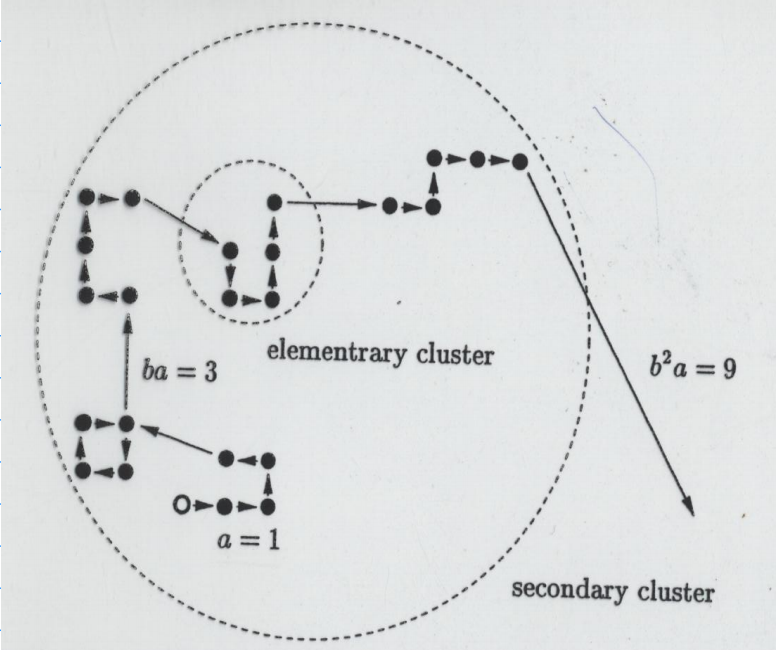
\includegraphics[width=0.4\textwidth]{figures/10_RWWeierstrass.png}
    \caption{\scriptsize Random Walk di Weierstrass ($b=3$, $M=4$): formazione dei Cluster (Paul and Baschangel: Stochastic Process, Springer).}
    \label{fig:figures-10_RWWeierstrass-png}
\end{figure}
\noindent
Proprio per la formazione di questi cluster su scale spaziali diverse il sistema può presentare un comportamento auto-similare.\\
Possiamo notare anche come cambiano i risultati al variare dei parametri $M$ e $b$:
\begin{figure}[H]
    \centering
    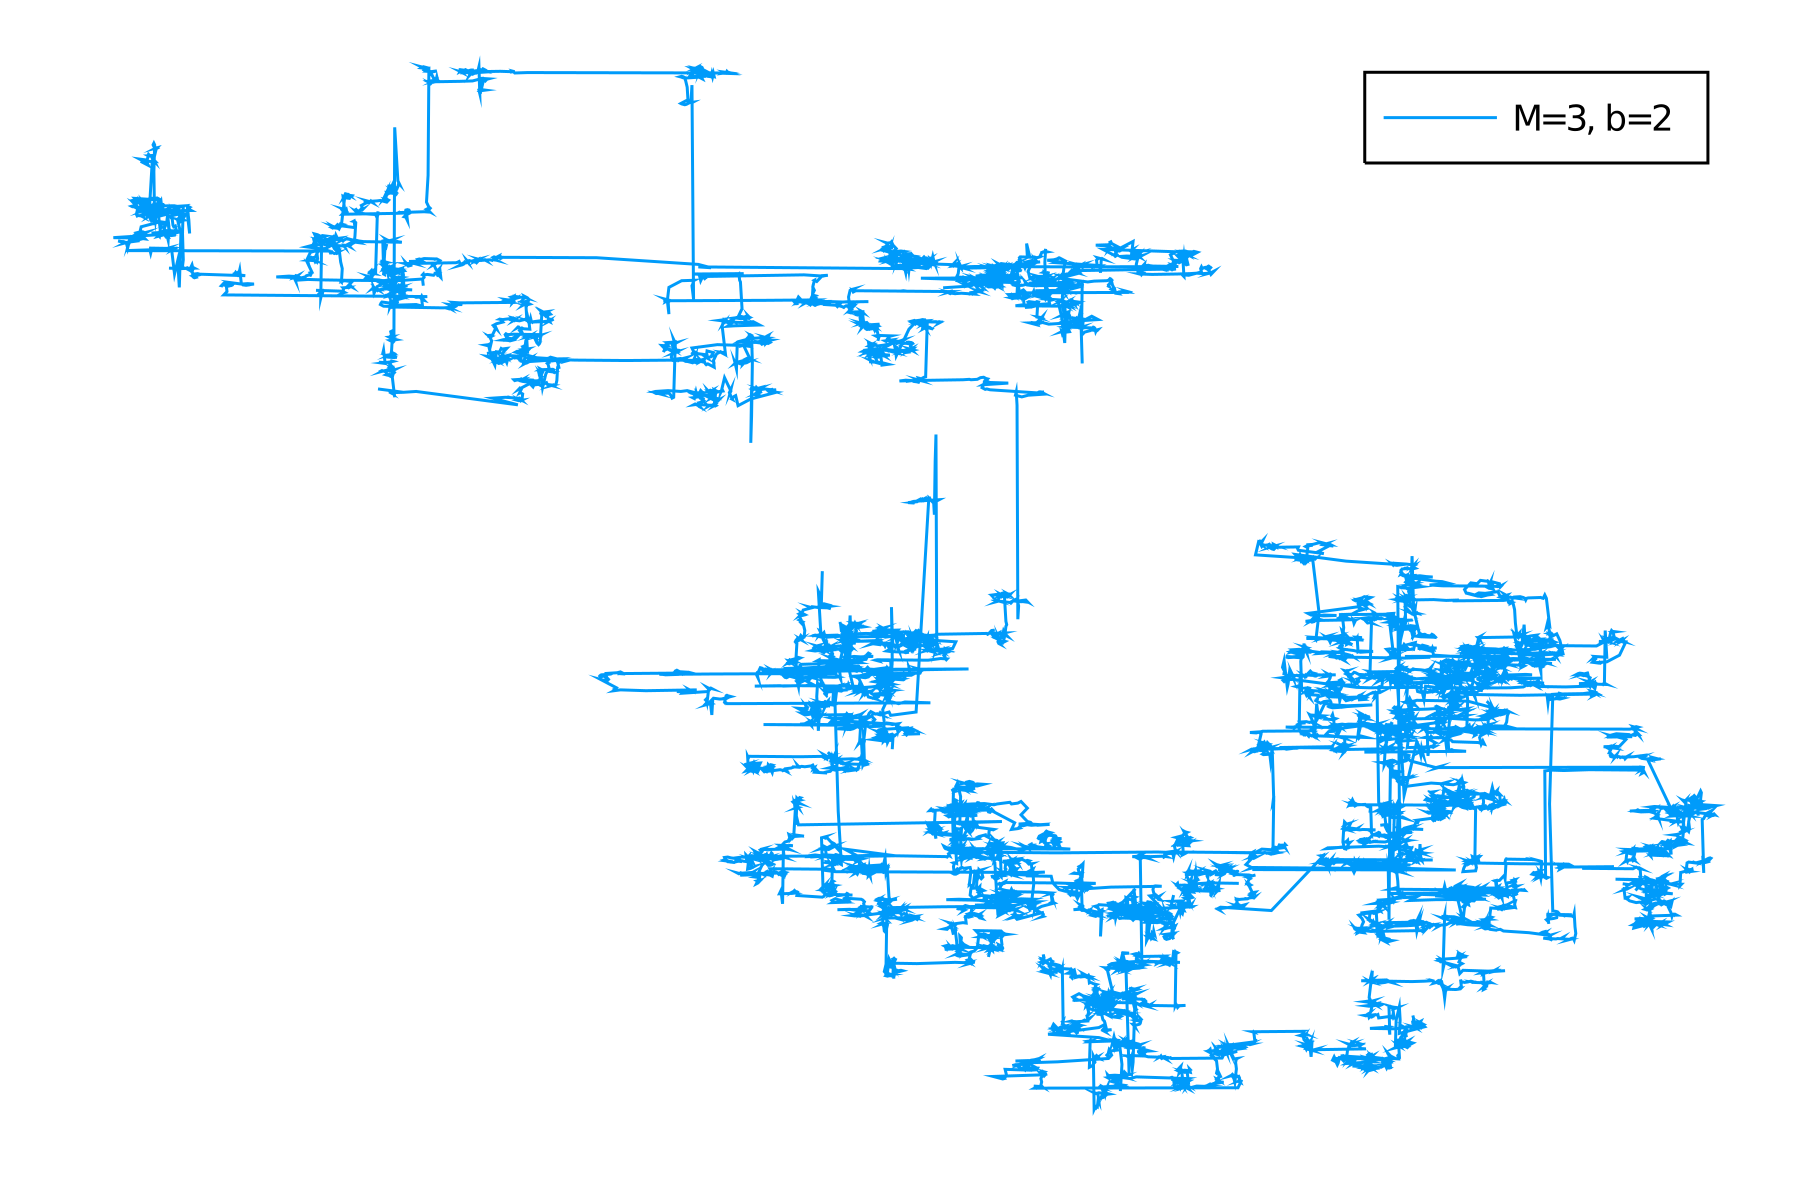
\includegraphics[width=0.45\textwidth]{figures/lez_10_Weier_M_3_b_2.png}
    \caption{\scriptsize Rapporto $M^2 / b = 4.5$.}
    \label{fig:figures-lez_10_Weier_M_3_b_2-png}
\end{figure}
\begin{figure}[H]
    \centering
    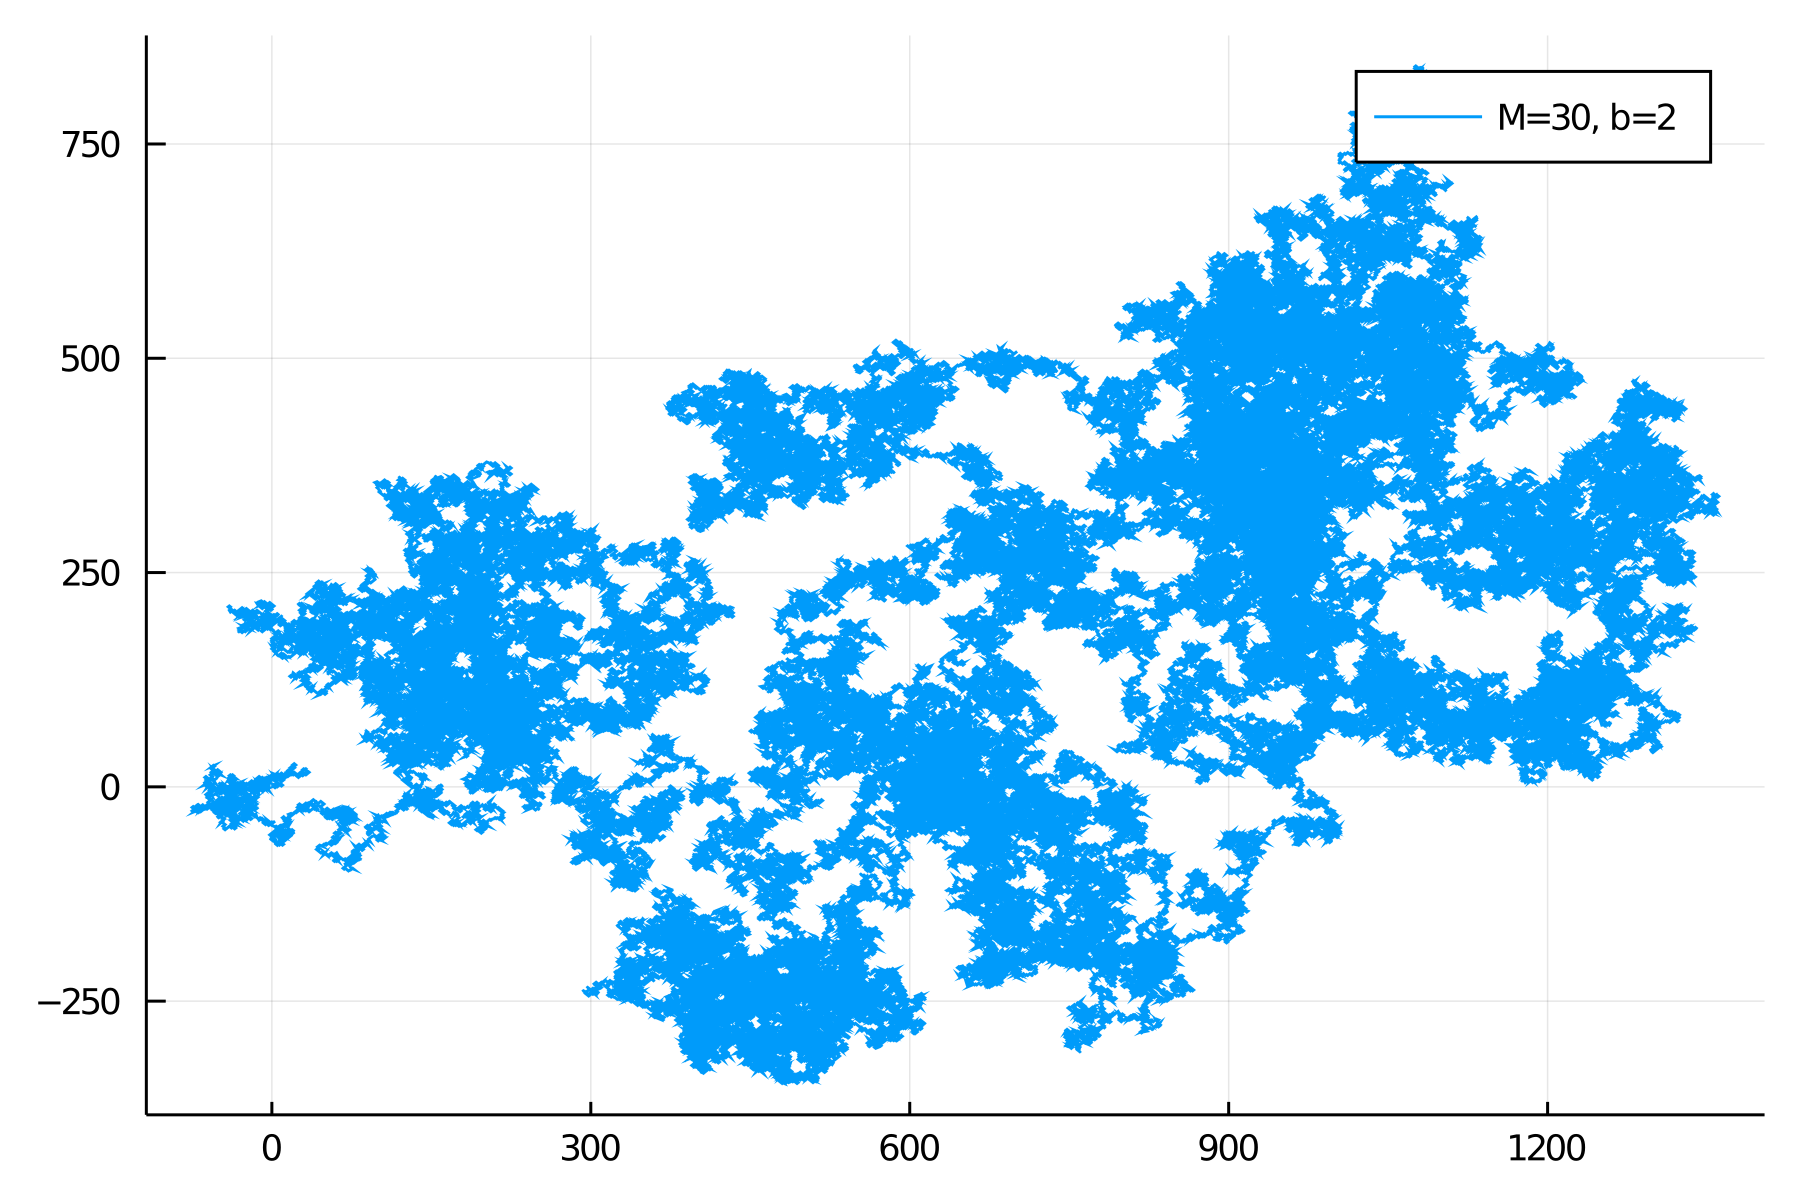
\includegraphics[width=0.45\textwidth]{figures/lez_10_Weier_M_30_b_2.png}
    \caption{\scriptsize Rapporto $M^2 / b = 450$, notiamo come i cluster che si formano siano diversi nei due casi.}
    \label{fig:figures-lez_10_Weier_M_3_b_2-png}
\end{figure}

Risolviamo per $\left<l^2\right>\to 0$, quindi il caso in cui la distribuzione $P(l)$  non può tendere ad una Gaussiana.
\[
    \left<l^2\right> = \frac{\left(M-1\right)a^2}{M}\sum_{}^{} \left(\frac{b^2}{M}\right)^J; \quad \frac{b^2}{M}>1
.\] 



\addtocounter{Sec}{\value{section}}%Mantengo il numero delle sezioni
\chapter{Sistemi caotici}
\setcounter{section}{\theSec}%Applico numero sezioni

\end{document}
